\documentclass[11pt]{book}
% alternative fonts: 
% times, mathptmx, mathpazo, newcent, bookman
% xref http://www.ce.cmu.edu/~kijoo/latex2pdf.pdf
\usepackage{newcent}
\usepackage{fullpage}
\usepackage{fancyvrb}
\usepackage[authoryear]{natbib}
\usepackage[pdftex]{graphicx}
\usepackage[backref,colorlinks]{hyperref}


% Typography.
\newcommand{\ccode}[1]{{\small\texttt{#1}}}
\newcommand{\emcode}[1]{{\small\bfseries\texttt{#1}}}
\newcommand{\prog}[1]{\small\texttt{#1}}
\newcommand{\eslmod}[1]{{\smaller\bfseries\texttt{#1}}}
\newcommand{\eslfunc}[1]{\hyperlink{man:#1}{{\small\texttt{#1}}}}

% Eliminate the ones below someday. 
\newcommand{\cmacro}[1]{\texttt{#1}}
\newcommand{\cvar}[1]{\texttt{#1}}
\newcommand{\cvartype}[1]{\texttt{#1}}
\newcommand{\cstruct}[1]{\texttt{#1}}
\newcommand{\cfunc}[1]{\texttt{#1}}
\newcommand{\cfile}[1]{\texttt{#1}}

\def\argmax{\mathop{\mathrm{argmax}}\limits}
\def\argmin{\mathop{\mathrm{argmin}}\limits}

\DefineVerbatimEnvironment{cchunk}{Verbatim}{fontsize=\scriptsize,xleftmargin=2.0\parindent}%

% Description-like environment for documenting functions/APIs.
% puts the description label in a minipage with a large hanging
% indent.
% Good christ this took a long time to develop.
% hanging indent trick stolen from Peter Wilson's hanging.sty @CTAN
% minipage allows multi-line label, and puts item on next line.
% customized list inspired by Kopka/Daly _Guide to LaTeX_ p.213
% SRE, Wed Dec 27 11:37:18 2000
%
\newenvironment{sreapi}{%
     \begin{list}{}{%
       \renewcommand{\makelabel}[1]{%
         \begin{minipage}{\textwidth}%
           \hangindent10em\hangafter1\noindent%
           {\bfseries\texttt{##1}\vspace{0.8em}}%
         \end{minipage}%
     }}}%
     {\end{list}}


% Description-like environment for producing lists like:
%
%     label  stuff, stuff, stuff
%
%    label2  more stuff, more stuff,
%            more stuff.
% \begin{sreitems}{Longest label} \item[label] stuff, ... \end{sreitems}
% SRE, Wed Dec 27 11:59:43 2000
%
\newenvironment{sreitems}[1]{%
     \begin{list}{}{%
       \settowidth{\labelwidth}{#1}%
       \setlength{\leftmargin}{\labelwidth}%
       \addtolength{\leftmargin}{\labelsep}%
       }}
     {\end{list}}


\begin{document}

\begin{titlepage}
{\Large

\vspace*{\fill}

\noindent
{\Huge{Easel}} \\ 
\rule[2pt]{\textwidth}{1pt} \\
\hspace*{\fill} {\large {A library of C functions for
    biosequence analysis} \\ }

\vspace*{\fill}

\begin{center}
\url{http://selab.janelia.org/easel/}\\
Version 0.1; May 2007 \\ 

\vspace*{\fill}

Sean Eddy\\
HHMI Janelia Farm Research Campus\\
19700 Helix Drive\\
Ashburn VA 20147\\
\url{http://selab.janelia.org/}\\
\end{center}

\vspace*{\fill}
}
\end{titlepage}

\vspace*{\fill}

\noindent 
Copyright (C) 2004-2005 HHMI/Washington University School of
Medicine.\\

\vspace{1.5em}
\noindent 
The Easel library, including both the software and its documentation,
is licensed and freely distributed under the Creative Commons
Attribution License.  To view a copy of this license, visit
\url{http://creativecommons.org/licenses/by/2.0/} or send a letter to
Creative Commons, 559 Nathan Abbott Way, Stanford, California 94305,
USA.



\newpage
\tableofcontents

\newpage
\chapter{Introduction}
\section{Overview of modules}
\begin{tabular}{llll}\hline
\textbf{Module} & \textbf{Description}       & \textbf{Requires} & \textbf{Augmentation(s)}\\\hline
  \multicolumn{4}{c}{\textbf{Core module}}\\
easel           & Framework for using Easel         &  -     & \\
  \multicolumn{4}{c}{\textbf{Foundation modules}}\\
alphabet        & Digitized biosequence alphabets   & easel  & \\
dmatrix         & Matrix algebra                    & easel  & \\ 
getopts         & Command line parsing              & easel  & \\
keyhash         & Keyword hashing                   & easel  & \\
msa             & Multiple sequence alignment i/o   & easel  & keyhash \\
parse           & Token-based file parsing          & easel  & \\
random          & Random number generator           & easel  & \\
regexp          & Regular expression matching       & easel  & \\
sqio            & Sequence file i/o                 & easel  & alphabet, msa\\
stack           & Pushdown stacks                   & easel  & \\
vectorops       & Vector operations                 & easel  & \\\hline
  \multicolumn{4}{c}{\textbf{Derived modules}}\\
bioparse\_paml  & PAML rate matrix datafiles        & easel dmatrix parse & \\
dirichlet       & Dirichlet densities               & easel gamma random & \\ 
gamma           & Gamma densities                   & easel random & \\
ratematrix      & Evolutionary rate matrices        & easel dmatrix vectorops & \\
wuss            & RNA structure annotation          & easel stack    & \\\hline
  \multicolumn{4}{c}{\textbf{Optional library interfaces}}\\
interface\_gsl    & GNU Scientific Library          & easel dmatrix & \\
interface\_lapack & LAPACK linear algebra library   & easel dmatrix & \\\hline
\end{tabular}



\section{Overview of data structures}

\begin{tabular}{lll}\hline
\textbf{Object}          & \textbf{Implemented in} & \textbf{Description}\\\hline
\ccode{ESL\_ALPHABET}    & \cfile{alphabet}        & Digitized sequence alphabet\\
\ccode{ESL\_DMATRIX}     & \cfile{dmatrix}         & 2D double-precision matrix for linear algebra \\
\ccode{ESL\_FILEPARSER}  & \cfile{parse}           & Simple token-based input file parser\\
\ccode{ESL\_GETOPTS}     & \cfile{getopts}         & Application configuration state\\
\ccode{ESL\_KEYHASH}     & \cfile{keyhash}         & Keyword hash table\\
\ccode{ESL\_MSA}         & \cfile{msa}             & Multiple sequence alignment\\
\ccode{ESL\_MSAFILE}     & \cfile{msa}             & Multiple sequence alignment file parser\\
\ccode{ESL\_PERMUTATION} & \cfile{dmatrix}         & Permutation matrix used in linear algebra\\
\ccode{ESL\_RANDOMNESS}  & \cfile{random}          & Random number generator\\
\ccode{ESL\_REGEXP}      & \cfile{regexp}          & Regular expression pattern-matching machine\\
\ccode{ESL\_SEQFILE}     & \cfile{sqio}            & Biosequence file parser (unaligned)\\
\ccode{ESL\_SQ}          & \cfile{sqio}            & DNA/RNA/protein sequence data\\
\ccode{ESL\_STACK}       & \cfile{stack}           & Pushdown stack\\\hline
\end{tabular}

\section{Module design}

Easel is designed to be used in two different ways: as a C library
(\ccode{libeasel.a}) in the usual C way, or by grabbing individual
source files without the rest of the library.

The ability to borrow individual files from Easel makes it different
from many other C libraries. For example, to get Easel's sequence file
i/o API, for example, you just take the sqio module (the C source
\ccode{esl\_sqio.c} and the header \ccode{esl\_sqio.h}), plus the
obligatory Easel core (\ccode{easel.c} and \ccode{easel.h}). Most of
Easel's modules can stand alone in this way (the \emph{base}
modules). Only a few are dependent on other modules (the
\emph{derived} modules), though even these can be used just by
bringing along the modules they depend on.

There are a couple of reasons to provide standalone capability. One
reason came from teaching a computational molecular biology
course. For homework programming assignments, I wanted to provide
students with simple .c files with well-documented APIs for routine
things like sequence i/o. This was to give them a head start, save
them from implementing boring things, and let them concentrate on
learning algorithms. But at the same time, I wanted them to be able to
see where the functionality was coming from, and to study the .c files
if they wanted, rather than treating the library as a black box -- so
I wanted to give them a few .c files at a time, not a library.

A second reason comes from my frustration with C libraries and code
reuse in bioinformatics in general. If I want to take a single routine
from someone's library (say, gods help us, the NCBI Toolkit), it's
common that that routine has dependencies, and the dependencies have
dependencies, and pretty soon I'm dragging the whole damned library in
just to have access to the routine I wanted. I don't mind that in
standard, widely installed system libraries, but if I'm making a
robustly distributable bioinformatics application, I need to include
in my package all my nonstandard dependencies -- and I really don't
want to have to distribute the entire GNU Scientific Library just to
pick up two GSL functions, all of LAPACK to get one numerical routine,
and the whole NCBI Toolkit to pick up one Toolkit routine.

Thus, Easel is very strictly modular in design. You never need the
entire Easel library to use any one aspect of Easel's
functionality. Most often, you need only the module you're interested
in, plus the core easel module.

To facilitate code reuse, Easel is licensed under a permissive open
source license (the Creative Commons Attribution License) that allows
you to freely modify and redistribute the code.

In the end, some of my original intent of providing simple
implementations as teaching examples has been lost. Rather than
providing two implementations (my intended simple teaching example and
a full-strength production example), Easel code is all production
code. But the modularity remains, and it seems to be useful in other
respects.  Modular design is just a Good Thing in general.  Easel
modules can be unit-tested in absence of the rest of the library.
And, though this remains to be seen, it should be easy for other
people to contribute modules and extend Easel, and it should be easy
for people to borrow and reuse Easel code.

\section{The ``augmentation'' concept}

The trouble with enforcing strict modular design is that while
\emph{you} (the application writer) can take advantage of any or all
of Easel's functionality as you wish, \emph{Easel} can't. An Easel
module, by design, is as isolated as possible from all other Easel
modules. It shouldn't use any functionality other than the essentials
in the core \eslmod{easel} module. But what if module X would benefit
from the cool features of module Y -- for instance, what if we want
the \eslmod{sqio} sequence i/o module to have access to the fast file
indexing capabilities of the \eslmod{ssi} module?  Start down this
road, and pretty soon the library is full of dependencies, the modular
design collapses, and we're back to a standard all-or-none C library.

Easel introduces a concept called \emph{augmentation}. The base
functionality of many Easel modules can be optionally \emph{augmented}
by one or more other Easel modules. An augmentation confers optional
powers on a module beyond its default standalone behavior.

Sometimes, an augmentation adds new functions to a module's API.  For
example, \eslmod{alphabet} augmentation of the sequence i/o module
\eslmod{sqio} adds a function to the \eslmod{sqio} API for digitizing
a sequence.

Sometimes, an augmentation extends or generalizes the scope of one or
more functions in the API. For instance, augmenting the \eslmod{sqio}
module with \eslmod{msa} gives the ability to read alignment files as
if they were sequential, unaligned sequence databases through
\eslmod{sqio}'s existing API.

And sometimes, an augmentation invisibly makes existing functions
faster or more memory-efficient, without adding any new functionality
per se.  For example, \eslmod{msa} can be augmented by
\eslmod{keyhash}, which makes the \eslmod{msa} module capable of
handling much larger alignments more efficiently than it does by
default, because \eslmod{keyhash} gives it the ability to use fast
hashing methods in its parsers.

When Easel is installed as a library, all modules are fully
augmented. This is done when the library is compiled. The
\ccode{configure} script automatically enables all augmentations when
it sets up the \ccode{easel.h} header, before compiling and installing
the library.

When you borrow an individual module from Easel, you choose whether to
borrow any modules that augment it. To activate an augmentation, you
not only have to compile and link the C code for the extra module
(obviously), you also edit a line in the \ccode{easel.h} header file
before compilation. There is a section at the top of \ccode{easel.h}
that declares which augmentations are to be enabled. You
\ccode{\#define} the appropriate flag for your augmentation to
activate it; for instance, to augment with \eslmod{ssi}, you make sure
\ccode{easel.h} has a line \ccode{\#define eslAUGMENT\_SSI} in place
of \ccode{\#undef eslAUGMENT\_SSI}.

Documentation for modules and their functions always distinguishes
between default functionality and augmented functionality.

\section{Function naming conventions in Easel}

\subsection{Object creation, initialization, destruction}

Most of Easel's objects are allocated on the heap; that is, accessed
exclusively via pointers. Less often, routines may allow an object to
be allocated on the stack.

\begin{sreitems}{\ccode{Create,Destroy}}
\item [\ccode{Create,Destroy}] 
  \ccode{esl\_foo\_Create()} allocates and initializes a new \ccode{ESL\_FOO}
  object, returning a pointer to the new
  object. The \ccode{Create()} function is passed any necessary
  initialization or size information in its arguments.
  \ccode{esl\_foo\_Destroy(obj)} frees all the memory associated
  with a \ccode{ESL\_FOO} object,  given a pointer to the object,
  and returns \ccode{ESL\_OK}. Example:

\begin{cchunk}
ESL_SQ *sq;

sq = esl_sq_Create();
esl_sq_Destroy(sq);
\end{cchunk}
  
\item [\ccode{Open,Close}] 
  Same as \ccode{Create()} and \ccode{Destroy()}, but specifically for
  objects associated with input/output streams. Example:

\begin{cchunk}
char        *seqfile = ``foo.seq'';
ESL_SIO     *sqfp;

sqfp = esl_sio_Open(seqfile);
esl_sio_Close(sqfp);
\end{cchunk}


\item [\ccode{Inflate,Deflate}]
  \ccode{esl\_foo\_Inflate(\&obj)} takes a pointer to the ``shell'' of an
  \ccode{ESL\_FOO} object that has been allocated on the stack, and
  allocates and initializes all the internals of it. The
  \ccode{Inflate()} function is passed any necessary initialization or
  size information in its arguments.  \ccode{esl\_foo\_Deflate(\&obj)}
  frees all the internal memory associated with a \ccode{ESL\_FOO} object,
  given a pointer to the object, but the object shell is left alone.
  The only difference between \ccode{Create,Destroy} and
  \ccode{Inflate,Deflate} is whether the object shell itself is to be
  allocated, or not. Example:

\begin{cchunk}
ESL_SQ  sq;

esl_sq_Inflate(&sq);
esl_sq_Deflate(&sq);
\end{cchunk}



\item [\ccode{Expand,Squeeze}]
   These deal with objects whose contents are not necessarily of a
   fixed size, but can grow and require reallocation of internal data
   fields. A function \ccode{esl\_foo\_Expand()} reallocates an
   \ccode{ESL\_FOO} object to a larger size. Usually, reallocation
   works by doubling the previous allocation. The redoubling strategy
   can result in a fair amount of unused memory overhead (up to
   50\%). A function \ccode{esl\_foo\_Squeeze()} takes a fully-grown
   object and optimizes its memory usage, recovering this wastage
   overhead, on the assumption that no more reallocation will be
   done.



\item [\ccode{Reuse}] 
   \ccode{esl\_foo\_Reuse(obj)} reinitializes an object exactly as a
   \ccode{Create} or \ccode{Inflate} function would initialize it, \emph{without}
   allocating new memory; it reuses memory that has
   already been allocated when the object was originally created or
   inflated. For some objects that are used sequentially (like,
   sequences), reusing one object saves malloc()'s compared to
   lots of Create/Destroy calls. A \ccode{Reuse} function does not
   care whether the object was originally created by a \ccode{Create}
   or a \ccode{Inflate} call. Example:

\begin{cchunk}
ESL_SQ *sq;

sq = esl_sq_Create();
  /* read a sequence into the sq object, have fun with it */

esl_sq_Reuse(sq);
  /* read a second sequence into it */

esl_sq_Destroy(sq);
\end{cchunk}

\end{sreitems}

\subsection{Other common object manipulation functions}

\begin{sreitems}{\ccode{\_Copy(src, dest)}}

\item[\ccode{\_Copy(src, dest)}]
Copies \ccode{src} object into \ccode{dest}, where the caller has
already created the empty \ccode{dest} object. Returns \ccode{ESL\_OK}
on success; throws \ccode{ESL\_EINCOMPAT} if the objects are not
compatible (for example, two matrices that are not the same size).

The order of the arguments is always \ccode{src} $\rightarrow$
\ccode{dest} (unlike the C library's \ccode{strcpy()} convention, which
is the opposite order).

\item[\ccode{\_Duplicate(obj)}] 

Creates and returns a pointer to a duplicate of \ccode{obj}.
Equivalent to (and is a shortcut for) \ccode{dest = \_Create();
\_Copy(src, dest)}. Caller is responsible for free'ing the duplicate
object, just as if it had been \ccode{\_Create}'d. Throws NULL if
allocation fails.

\item[\ccode{\_Set*(obj, value...)}]

Initializes value(s) in \ccode{obj} to \ccode{value}. Special cases of
\ccode{\_Set*} functions may exist, like \ccode{\_SetZero} (set to
zero(s)), or \ccode{esl\_dmatrix\_SetIdentity} (set a dmatrix to an
identity matrix).

\end{sreitems}


\section{Discipline of writing Easel modules}


\subsection{API}

\begin{enumerate}
\item Exposed function names obey Easel conventions.

\item All \ccode{ret\_*} pointers for retrieving info from 
      a function are implemented as optional.

\item On any error (returned or thrown), a function releases any
      memory it has allocated, and all \ccode{ret\_*} pointers are
      \ccode{NULL} or 0, depending on their type.

\item Any function that calls another Easel function must 
      catch any thrown errors. Within Easel, we
      can't assume that the error handler is set to be a fatal
      one.
\end{enumerate}


\subsection{Documentation}

\begin{enumerate}
\item Documentation in .tex files is written to application developers
      (and me); documentation in .c comments is written to Easel
      developers (and me).

\item Every module has a .tex file documenting the module and its API,
      and (if it makes sense) also the particular implementation.

\item Every function exposed to the API can be autodocumented (comment
      header can be converted to \LaTeX) with
      \ccode{autodoc\_functions}, in order to produce appendices
      summarizing the complete Easel function set.
\end{enumerate}


\subsection{Testing}

\begin{enumerate}

\item Every module has a test driver which exercises the API in some
      simple way (and, in the process, provides a ``hello world''
      level example of using the module).

\end{enumerate}











\vspace*{\fill}
\begin{quote}
\emph{Lack of skill dictates economy of style.} \hspace{3em} -- Joey Ramone
\end{quote}     

\newpage
\chapter{Core modules}

\section{The easel (esl) module: error handling and other fundamentals}
The easel (esl) module implements a small set of functionality shared
by all the modules: notably, the error-handling system.

\subsection{Error handling}

Easel is intended for use in applications ranging from quick \& dirty
one-off command line applications to complex graphical user interfaces
and parallel systems. Simple and complex applications have different
views of how errors and exceptions should be handled by a library.  On
the one hand, a robust application wants a guarantee that execution
never terminates within a library routine; control should be returned
to the application even in the most dire and unexpected
circumstances. We don't want Easel to crash a whole graphical user
environment, for example. And because an application is not
necessarily associated with a terminal, Easel cannot print error
messages directly to \emph{stderr}; \emph{stderr} may not go anywhere
useful. On the other hand, a quick \& dirty command line application
doesn't want to use lots of code checking for various dire and
unexpected errors. It would prefer to have Easel crash out with an
appropriate message to \ccode{stderr} -- that's all a simple
application would do anyway.

Easel processes all \textbf{exceptions} with one function,
\eslfunc{esl\_error()}, which takes an error code, error message,
source file name, and source line number as arguments.
\eslfunc{esl\_error()}, hands this information to a customizable error
handling function. The default error handler is a fatal one, which
performs the simple behavior: it prints the error message to
\ccode{stderr} and aborts execution. Therefore, by default,
applications can rely on Easel to handle its own exceptions.  In an
application that wants to handle all exceptions itself, and wants a
guarantee that execution will never terminate from within Easel, a
custom nonfatal error handler can be assigned to \eslfunc{esl\_error()},
one which merely catches the information from Easel (and reacts
appropriately) but returns control to Easel at the point of
failure. Easel percolates the error code up through its call stack
until control returns to your application with an appropriate nonzero
error code. \footnote{The idioms used in Easel to handle serious
exceptions non-fatally look a lot like exception handling in more
modern languages like C++/Java.}

Easel distinguishes exceptions from \textbf{normal errors}. ``Normal''
errors are conditions that any application should handle gracefully,
even a simple application. One example is an end-of-file indicator
from an input routine. Most importantly, any problem that is the fault
of the user (typo in a command line argument, bad file format, and
suchlike) is called a normal error. (Bad user input is ``normal''. It
should not crash a program with an exception.) Easel functions handle
normal errors by directly returning an appropriate nonzero status code
to the caller, without sending a message through the handler in
\eslfunc{esl\_error()}. A limitation of this approach is that your
application only gets a status code, not a message, when a normal
error occurs. Often the status code is sufficient for your application
to know what happened. For instance, \ccode{eslEOF} means end-of-file,
so your application might report \ccode{"premature end of file"} if it
receives such a status code unexpectedly. But when the error involves
a file format syntax problem (for instance) a terse \ccode{eslESYNTAX}
return code is not as useful as knowing \ccode{\"Parse failed at line
42 of file foo.data: expected integer, got 'boo!'\"}. File parsers in
Easel are generally encapsulated in objects; these objects include a
\ccode{errbuf[]} string that contains a useful error message when a
parser function returns a normal error. (For instance, see the
\eslmod{sqio} module and its \ccode{ESL\_SQFILE} object for sequence
file parsing.)

Easel also distinguishes a third class of error, termed
\textbf{violations}. Violations are bugs: problems that should never
arise in production code, and that should be caught during development
and testing. Violations result in an \ccode{abort()} and immediate
program termination; therefore, they never occur in production
code. They are generated by two mechanisms: from assertions that can
be optionally enabled in development code, or from test harnesses that
call the always-fatal \eslfunc{esl\_fatal()} function when they detect a
problem they're testing for. For example, Easel uses conditionally
compiled assertions to test for violations of Easel's API design
contracts. \footnote{``Design-by-contract'' is a useful software
engineering concept introduced by the Eiffel language
[\url{www.eiffel.com}]. C does not inherently support DBC, but Easel
partially emulates it using assertions.}

\subsubsection{Error handling: application perspective}

Almost all Easel functions return an integer status code, where
\ccode{eslOK} (0) indicates success and a nonzero code indicates a
failure. The list of status codes is shown in
Table~\ref{tbl:statuscodes}.

\begin{table}
\begin{center}
\input{cexcerpts/statuscodes}
\end{center}
\caption{List of all status codes that might be returned by Easel functions.}
\label{tbl:statuscodes}
\end{table}

There are some exceptions. Some \ccode{*_Create()} functions that
allocate and create new objects follow a convention of returning a
valid pointer on success, and \ccode{NULL} on failure; these are
functions that only fail by memory allocation failure. Destructor
functions (\ccode{*_Destroy()}) always return \ccode{void}, and must
have no points of failure of their own, because destructors can be
called when we're already handling an exception. Finally, there are
some functions that simply return an answer, rather than a status
code; these must be functions that have no failure points. Easel is
not completely dogmatic.

Documentation of individual Easel functions refers to exceptions that
are handled by \eslfunc{esl\_error()} as \textbf{thrown}, and normal
error conditions that directly return an error status code as
\textbf{returned}.  From the perspective of an application developer
using Easel, any \emph{returned} error codes \textbf{must} always be
checked. Moreover, a function's documentation always lists all
possible return codes that you need to deal with.  In contrast, a
simple application does not need to pay attention to thrown exceptions
at all. The default error handler deals with them (fatally). However,
an application that registers a custom nonfatal error handler does
need to check for both returned errors and thrown exceptions. Although
each function's documentation \emph{in principle} lists all thrown
exceptions, \emph{in practice}, an application developer should not
trust this list. Because exceptions may percolate up from other Easel
calls, it is easy to forget to document all possible
exceptions.\footnote{If we combined a static code analyzer with a
script that understands Easel's exception conventions, we could
automate the enumeration of all possible codes. This would be a Good
Thing to do in the future.} An application that's catching exceptions
should always have a failsafe catch for any nonzero return status. For
example, a minimal try/catch idiom for an application calling a Easel
function is something like:

\begin{cchunk}
     int status;
     if ((status = esl_foo_function()) != eslOK)  my_failure_function();
\end{cchunk}

A little more complex one that catches some specific errors, but has a
failsafe for everything else, is:

\begin{cchunk}
     int status;
     status = esl_foo_function();
     if      (status == eslEMEM) my_failure("Memory allocation failure");
     else if (status != eslOK)   my_failure("Unexpected exception %d\n\", status);
\end{cchunk}

Finally, the exception-catching idiom used in Easel's own source is
one way of consistently cleaning up and guaranteeing a certain state
upon failure, before percolating an exception code upwards:

\begin{cchunk}
     int status;
     if ((status = esl_foo_function()) != eslOK)  goto FAILURE;
     ... do other stuff...
     return eslOK;

  FAILURE:
     free(whatever);
     set(any return variables);
     return status;
\end{cchunk}


\subsubsection{Replacing the default error handler}

\eslfunc{esl\_error()} gets as arguments a status code, file and
linenumber for where the error occurred, and a \cfunc{printf()}-style
message. By default, it prints the message and exits:

\begin{cchunk}
Easel fatal error:
Memory allocation failed.

Aborted at file sqio.c, line 42. 
\end{cchunk}

An application can define its own handler for the same information,
and override this default behavior. To do this, you define the error
handler with the following prototype:

\begin{cchunk}
extern void my_error_handler(int code, char *file, int line, char *format, va_list arg);
\end{cchunk}

An example implementation of an error handler:

\begin{cchunk}
#include <stdarg.h>

void
my_error_handler(int code, char *file, int line, char *format, va_list arg)
{
  fprintf(stderr, ``Easel threw an error (code %d):\n'', code);
  vfprintf(stderr, format, arg);
  fprintf(stderr, ``at line %d, file %s\b'', line, file);
  return;
}
\end{cchunk}

To configure Easel to use your error handler, call
\eslfunc{esl\_error\_SetHandler(\&my\_error\_handler)}. Normally you
would do this before calling any other Easel functions.

However, in principle, you can change error handlers at any time --
including restoring the default handler with
\eslfunc{esl\_error\_RestoreDefaultHandler()}.  The implementation of
the handler relies on a static function pointer that is not
threadsafe, so if you are writing a threaded program, you want to make
sure that multiple threads do not try to change the handler at the
same time.

Because Easel functions may call other Easel functions, the function
that first detects an error may not be the function that your
application called.  If you implement a nonfatal handler, an abnormal
error in Easel may generate a partial stack trace of
\eslfunc{esl\_error()} messages, as the exception percolates up from
the function that detected the error, until control finally returns to
your application. Your error handler should deal with the possibility
of this stack trace. The first \eslfunc{esl\_error()} message is most
relevant, and subsequent messages arise from that error percolating up
through the stack trace.  For example, a sophisticated replacement
\eslfunc{esl\_error()} handler might push each \eslfunc{esl\_error()}
message into a FIFO queue, where they will be waiting for a main
application-specific error handler to access when your application
gets its thrown exception code back from Easel.

\subsubsection{Internal API for exception handling}

You only need to understand this section if you want to understand
Easel's source code (or other code that uses Easel conventions, like
HMMER), or if you want to use Easel's error conventions in your own
source code.

Throwing an exception involves two or three steps. The first is a call
to \eslfunc{esl\_error()} with a status code, \ccode{\_\_FILE\_\_} and
\ccode{\_\_LINE\_\_} information, and an error message. The second (if
necessary) is to clean up and set the failure state (which may include
free'ing allocated memory, restoring an object to its original state,
and setting any returned variables to the values they should have on
failure). The third is to return the error code.

Two wrapper macros implement this convention for almost all
exceptions: \eslfunc{ESL\_ERROR()} and \eslfunc{ESL\_FAIL()}. They are
defined in \ccode{easel.h} as:

\begin{cchunk}
\input{cexcerpts/error_macros}
\end{cchunk}

\eslfunc{ESL\_ERROR()} is the simpler version for when cleanup isn't
necessary. It just calls \eslfunc{esl\_error()} and returns the status
code. \eslfunc{ESL\_FAIL()} implements the three-step version when a
cleanup is needed before the return. It is an offensive little
abomination, because it's not self-contained. It requires an
\ccode{int status} variable in scope, a \ccode{FAILURE:} target for
the \ccode{goto} - and it uses a \ccode{goto}. But if you can stomach
that, it provides for a fairly clean idiom for catching exceptions and
cleaning up, and cleanly setting different return variable states on
success versus failure, as illustrated by this pseudoexample:

\begin{cchunk}
int 
foo(char **ret_buf, char **ret_fp)
{
    int status;
    char *buf = NULL;
    FILE *fp  = NULL;

    if ((buf = malloc(100))  == NULL) ESL_FAIL(eslEMEM,      "malloc failed");
    if ((fp  = fopen("foo")) == NULL) ESL_FAIL(eslENOTFOUND, "file open failed");

    *ret_buf = buf;
    *ret_fp  = fp;
    return eslOK;

  FAILURE:
    if (buf != NULL) free(buf);  *ret_buf = NULL;
    if (fp  != NULL) fclose(fp); *ret_fp  = NULL;
    return status;
}
\end{cchunk}

After a lot of putzing about with different conventions, I think that
might be about as clean as you can make exception handling in C. An
alternative is to actually implement \ccode{try} and \ccode{catch},
using \ccode{setjmp()}/\ccode{longjmp()}, but I don't find such code
to be very pretty.

For memory allocation and reallocation, Easel also uses two macros
\eslfunc{ESL\_ALLOC()} and \eslfunc{ESL\_RALLOC()}, which encapsulate
standard \eslfunc{malloc()} and \eslfunc{realloc()} calls in Easel's
error-throwing convention.



\vspace*{\fill}
\begin{quote}
\emph{Only a complete outsider could ask your question. Are there
control authorities? There are nothing but control authorities. Of
course, their purpose is not to uncover errors in the ordinary meaning
of the word, since errors do not occur and even when an error does in
fact occur, as in your case, who can say conclusively that it is an
error?} \hspace{3em} -- Franz Kafka, in \emph{The Castle}
\end{quote}     

\newpage
\section{The alphabet (abc) module: digitized biosequences}
The \eslmod{alphabet} module contains routines for digitizing
alphabetic biosequences.



It is convenient to represent nucleotides and amino acids as array
indices 0..3 or 0..19, respectively, for efficiency as well as other
reasons. It is also convenient to index biosequences in 1..L
coordinates instead of the C language's 0..L-1 array representation,
in part for human readability, and also because some codes (dynamic
programming alignment algorithms, for example) have boundary
conditions where initializing a boundary at coordinate 0 is
convenient.

Real biosequences do not consist of just four or twenty different
canonical symbols, though. The \eslmod{alphabet} module also provides
mechanisms for dealing with several other biosequence coding issues:

\begin{itemize}
  \item Degenerate residue symbols representing uncertainties,
        including both IUPAC/IUBMB standard one-letter nomenclature
        and nonstandard extensions such as the use of \ccode{J} to
        mean isoleucine or leucine (\ccode{I|L}) in protein sequences
        determined by mass spec;

  \item Standard and nonstandard symbols for unusual residues, such as
        selenocysteine (\ccode{U}) and pyrrolysine (\ccode{O}) in
        proteins ;

  \item \emph{Ad hoc} symbols representing modified residues, such as
        the slew of one-letter codes used to annotate
        posttranscriptionally modified nucleotides in the Sprinzl tRNA
        database \citep{Sprinzl98};

  \item Case-insensitivity of input sequences, for instance allowing
        both \ccode{a} and \ccode{A} to mean alanine in amino acid
        sequences;

  \item Tolerating common malpractices, like the use of \ccode{X}
       instead of \ccode{N} as a degeneracy code in nucleic acid
       sequence;

  \item The semantic difference between a gap symbol and a missing
        data symbol in sequence alignments.
\end{itemize}        

The \eslmod{alphabet} module provides standard defaults for protein,
RNA, and DNA alphabets which follow both community standards and
IUPAC/IUBMB nomenclature for representing sequence residues in
one-letter ASCII characters. Additionally, the design of the
\eslmod{alphabet} module is flexible enough to allow an application to
customize its own alphabet, to deal with these issues almost any way
it chooses.

Table~\ref{tbl:alphabet_api} lists the functions in the
\eslmod{alphabet} API.  Easel maintains alphabet information in an
\ccode{ESL\_ALPHABET} structure. An application usually creates its
alphabet once, possibly even as a global variable.  A digitized
sequence \ccode{dsq} is an \ccode{unsigned char *} array of length
\ccode{L+2}, where \ccode{dsq[1..L]} are digitized residues, and
\ccode{dsq[0]} and \ccode{dsq[L+1]} are sentinel bytes (of value
\ccode{eslSENTINEL}, 127).

\begin{table}[hbp]
\begin{center}
\begin{tabular}{ll}\hline
   \multicolumn{2}{c}{\textbf{The \ccode{ESL\_ALPHABET} object}}\\
\ccode{esl\_alphabet\_Create()}       & Create alphabet of standard type. \\
\ccode{esl\_alphabet\_CreateCustom()} & Create a custom alphabet. \\
\ccode{esl\_alphabet\_SetEquiv()}     & Define an equivalent symbol. \\
\ccode{esl\_alphabet\_SetCaseInsensitive()} & Make a custom alphabet case insensitive. \\
\ccode{esl\_alphabet\_SetDegeneracy()} & Define degenerate symbol in custom alphabet. \\
\ccode{esl\_alphabet\_Destroy()}      & Frees an alphabet object. \\
   \multicolumn{2}{c}{\textbf{Digitized sequences}}\\
\ccode{esl\_dsq\_Create()}       & Allocate and create a new \ccode{dsq}. \\
\ccode{esl\_dsq\_Set()}          & Digitize a sequence into existing \ccode{dsq} space. \\
   \multicolumn{2}{c}{\textbf{Other functions}}\\
\ccode{esl\_abc\_\{I,F,D\}AvgScore()}  & Calculate avg score of degenerate residue.\\
\ccode{esl\_abc\_\{I,F,D\}ExpectScore()} & Calculate expected score of degenerate residue.\\
\ccode{esl\_abc\_Type()}               & Convert internal alphabet type code to output string.\\
\ccode{esl\_abc\_\{F,D\}Count()}       & Count a digital symbol towards a countvector.\\
\ccode{esl\_abc\_DigitizeSymbol()}     & Returns digital code for one ASCII character.\\
\ccode{esl\_abc\_XIsDegenerate()}      & Returns TRUE given code for a degeneracy.\\
\ccode{esl\_abc\_XIsBasic()}           & Returns TRUE given code for a fundamental residue.\\
\ccode{esl\_abc\_XIsGap()}             & Returns TRUE given code for a gap.\\
\ccode{esl\_abc\_CIsDegenerate()}      & Returns TRUE given a degenerate character.\\
\ccode{esl\_abc\_CIsBasic()}           & Returns TRUE given a fundamental residue.\\
\ccode{esl\_abc\_CIsGap()}             & Returns TRUE given a gap character.\\

\hline
\end{tabular}
\end{center}
\caption{The \eslmod{alphabet} API.}
\label{tbl:alphabet_api}
\end{table}

\subsection{An example of using the alphabet API}

Figure~\ref{fig:alphabet_example} shows an example of creating a DNA
alphabet and digitizing a short DNA sequence.

\begin{figure}
\input{cexcerpts/alphabet_example}
\caption{An example of using the \eslmod{alphabet} module.}
\label{fig:alphabet_example}
\end{figure}

\begin{itemize}
\item A standard biosequence alphabet is created using
\ccode{esl\_alphabet\_Create(type)}, where \ccode{type} can be
\ccode{eslDNA}, \ccode{eslRNA}, or \ccode{eslAMINO}.

\item An input sequence \ccode{seq} of length \ccode{L} is digitized
according to alphabet \ccode{a}, creating a newly allocated digital
sequence \ccode{dsq}, by calling \ccode{esl\_dsq\_Create(a, seq, L,
\&dsq)}. The caller must free \ccode{dsq} using \ccode{free(dsq)}.
Alternatively, if the caller has already allocated \ccode{L+2} (or
more) bytes in \ccode{dsq}, it can call \ccode{esl\_dsq\_Set(a, seq,
L, dsq)}, which is the non-allocating version of
\ccode{esl\_dsq\_Create()}.

\item For an input sequence of length \ccode{L}, the digitized
sequence \ccode{dsq} is a \ccode{char *} array of \ccode{L+2}
bytes. \ccode{dsq[0]} and \ccode{dsq[L+1]} contain a sentinel byte of
value \ccode{eslSENTINEL} (127).  Positions \ccode{1..L} hold the
residues, where values \ccode{0..3} encode \ccode{ACGT} in DNA
sequences, \ccode{0..3} encode \ccode{ACGU} in RNA sequences, and
\ccode{0..19} encode \ccode{AC..WY} in amino acid sequences.

\item Both sequence-digitizing functions return \ccode{eslEINVAL} if
the input sequence contains characters that are not in the
alphabet. Because input sequences are often provided by a user (not
the program), this is a common error that the application must check
for.
\end{itemize}

\subsection{Concepts and terminology}

A \esldef{symbol} is a 7-bit ASCII input character, representing a
residue, gap, or degeneracy. A \esldef{code} is the digital internal
representation of the symbol as an \ccode{unsigned char} in the range
$0..127$, suitable for use as an array index. The \eslmod{alphabet}
module translates input symbols into internal digital codes.

We distinguish between an input alphabet, an internal alphabet, and a
canonical alphabet.  The \esldef{input alphabet} consists of all the
symbols that Easel allows in an input biosequence character
string. The \esldef{internal alphabet} is the standardized one-letter
alphabet that Easel deals with. The \esldef{canonical alphabet} is the
fundamental set of 4 nucleotides or 20 amino acids.

Easel deals with all of the complications of sequence encoding using
two concepts, equivalency and degeneracy.  \esldef{Equivalency}
defines how the input alphabet maps to the internal
alphabet. \esldef{Degeneracy} defines how the internal alphabet maps
to the canonical alphabet.

Equivalent residues are symbols that are accepted in an input sequence
character string and silently translated into an appropriate internal
code. Characters in the input alphabet are mapped many-to-one to the
internal alphabet using an \esldef{input map}. One use of equivalency
is to map both lower and upper case input to the same internal
symbol. Another use is to allow several different input characters to
mean a gap. Another use is to silently accept and ``fix'' nonstandard
but common input ``errors'', such as tolerating the use of X to mean N
in nucleic acid sequences.

Degenerate residues are codes in the internal alphabet that are mapped
one-to-many onto canonical residue codes, using a \esldef{degeneracy
map}. In addition to mapping the degeneracy codes onto the canonical
alphabet, the degeneracy mechanism is also used to deal with unusual
and modified residues. Selenocysteine, for instance, is represented by
default as a \ccode{U}, but treated as a degenerate code for \ccode{C}
(cysteine). The rationale for this will be described in more detail
below.

\subsubsection{The internal alphabet}

Easel's internal alphabet is a string (\ccode{a->sym}) of length
\ccode{Kp}, which contains:

\begin{itemize}
 \item the \ccode{K} symbols of the canonical alphabet;
 \item a standard gap symbol;
 \item (optionally) any other degenerate, unusual, or modified residue codes;
 \item a mandatory ``any'' symbol (a completely degenerate residue);
 \item a standard ``missing data'' symbol.
\end{itemize}

Residues \ccode{0..K-1} must be the canonical alphabet.  Residue
\ccode{K} must be the gap symbol.  Residues \ccode{K+1..Kp-3} must be
the degenerate and modified residue symbols (there can be zero of
these). Residue \ccode{Kp-2} must be the completely degenerate symbol
(such as \ccode{X} for protein sequence or \ccode{N} for nucleic acid
sequence); all alphabets must have such a symbol. Residue \ccode{Kp-1}
must be the missing data symbol.  Because the completely-degenerate
symbol and the two kinds of gap symbols are mandatory in any alphabet,
\ccode{Kp} $\geq$ \ccode {K+3}. Aside from these constraints, symbols
may occur in any order.

The digital code used for each residue is then the index of a residue
in this string, \ccode{0..Kp-1}. The only other value that can appear
in a digitized sequence is \ccode{eslSENTINEL} (127), the sentinel
byte in positions \ccode{0} and \ccode{L+1} of a digitized sequence of
length \ccode{L}. 

The rationale for the ordering is the following. Most applications
will define residue scores in vectors and matrices that are smaller
than the full range of the internal alphabet; for instance, it's
common to only have \ccode{K} scores for the canonical residues.  As
much as possible, we want array indices to be the same whether we're
accessing the full internal alphabet or a smaller score vector or
matrix. So: we expect many applications to have score vectors or
matrices that only contain the \ccode{K} canonical residues, so the
canonical residues go first.  We expect some applications to treat
gaps as an extra symbol, and provide \ccode{K+1} position-specific
scores or a \ccode{K+1} $\times$ \ccode{K+1} score matrix, so the gap
character is next. We expect a few applications to optimize degeneracy
scoring by precalculating them in \ccode{Kp-1} vectors or $Kp-1 \times Kp-1$
matrices, so the degeneracies go next (the gap character at $K$ might
then go unused in the score vectors and matrices, but that's a minor
inefficiency).  The missing data symbol is expected to always require
special handling when it occurs, rather than appearing in a score
vector or matrix, so it's put last.

\subsection{The standard alphabets: DNA, RNA, protein}

The three standard internal alphabets are:

\begin{table}[h]
\begin{tabular}{llccrr}
\textbf{Type} & \ccode{sym}  & \textbf{equivs} & \textbf{gaps}   & \ccode{K} & \ccode{Kp} \\
\ccode{eslRNA}        & \ccode{ACGU-RYMKSWHBVDN\~}            & T=U; X=N & \ccode{-\_.} & 4         &  17         \\
\ccode{eslDNA}        & \ccode{ACGT-RYMKSWHBVDN\~}            & U=T; X=N & \ccode{-\_.} & 4         &  17         \\
\ccode{eslAMINO}      & \ccode{ACDEFGHIKLMNPQRSTVWY-BJZOUX\~} &          & \ccode{-\_.} & 20        &  28         \\
\end{tabular}
\end{table}

The \ccode{sym} string contains all the symbols that can be handled
internally, and all the residues that can be represented when a
digitized sequence is converted back to text. An application might
still convert some characters for its own purposes before displaying
an alphabetic string; for instance, to use different gap symbols for
insertions versus deletions, or to use upper/lower case conventions to
represent match/insert positions in a profile HMM alignment.

The standard DNA and RNA alphabets follow published IUBMB
recommendations (``Nomenclature for incompletely specified bases in
nucleic acid'' \citep{IUBMB85}), with an addition of X as an
equivalence for N (acquiescing to the \emph{de facto} BLAST filter
standard of using X's to mask residues), and equivalencing T to U in
RNA sequences (and vice versa in DNA).

The one-letter code for amino acids follows section 3AA-21 of the
IUPAC recommendations \citep{IUPAC84}. The code is augmented by U for
selenocysteine, as recommended in 1999 by the JCBN/NC-IUBMB Newsletter
(\url{http://www.chem.qmul.ac.uk/iubmb/newsletter/1999/item3.html}).
It is also augmented by O for pyrrolysine and J for a
leucine/isoleucine ambiguity (from a mass spectrometry experiment),
following usage in the RESID database
(\url{http://www.ebi.ac.uk/RESID/}).


\subsection{Degenerate residues}

The symbols from \ccode{K+1..Kp-3} in the internal alphabet are all
treated as degenerate residues.

When creating a custom alphabet, each degenerate symbol is initialized
by calling \ccode{esl\_alphabet\_SetDegeneracy(alphabet, c, syms)} to
assign degenerate alphabetic symbol \ccode{c} to the alphabetic
symbols in the string \ccode{syms}. For example,
\ccode{esl\_alphabet\_SetDegeneracy(a, 'R', \"AG\")} assigns R
(purine) to mean A or G.  For the standard biosequence alphabets, this
is done automatically to define the proper degeneracy codes.

For amino acid alphabets, the default code is:

\begin{cchunk}  
  esl_alphabet_SetDegeneracy(a, 'B', "ND");
  esl_alphabet_SetDegeneracy(a, 'J', "IL");
  esl_alphabet_SetDegeneracy(a, 'Z', "QE");
\end{cchunk}

For RNA alphabets, the default code is:

\begin{cchunk}
  esl_alphabet_SetDegeneracy(a, 'R', "AG");
  esl_alphabet_SetDegeneracy(a, 'Y', "CU");
  esl_alphabet_SetDegeneracy(a, 'M', "AC");
  esl_alphabet_SetDegeneracy(a, 'K', "GU");
  esl_alphabet_SetDegeneracy(a, 'S', "CG");
  esl_alphabet_SetDegeneracy(a, 'W', "AU");
  esl_alphabet_SetDegeneracy(a, 'H', "ACU");
  esl_alphabet_SetDegeneracy(a, 'B', "CGU");
  esl_alphabet_SetDegeneracy(a, 'V', "ACG");
  esl_alphabet_SetDegeneracy(a, 'D', "AGU");  
\end{cchunk}

For DNA alphabets, the calls are is the same as for RNA code, but with
\ccode{T} in place of \ccode{U}.


\subsubsection{Implementation: the degeneracy map}

The alphabet's degeneracy map is implemented in an array
\ccode{a->degen[0..Kp-1][0..K-1]} of 1/0 (TRUE/FALSE) flags.
\ccode{a->degen[x][y] == TRUE} indicates that the residue set $D(x)$
for degeneracy code \ccode{x} contains base residue \ccode{y}.
\ccode{a->ndegen[x]} contains the cardinality $|D(x)|$, how many base
residues are represented by degeneracy code \ccode{x}.

For the two kinds of gap symbols, the degeneracy map is empty; all
flags are FALSE and the cardinality is 0.

Because character \ccode{Kp-3} in the internal alphabet is
automatically assumed to be an ``any'' character (such as 'N' for DNA
or RNA, 'X' for protein), \ccode{a->degen[Kp-3][i] = 1} for all
$i=0..K-1$, and \ccode{a->ndegen[Kp-3] = K}.

The storage of the degeneracy map is a little wasteful. We really only
need rows \ccode{a->degen[K+1..Kp-3]}, but optimizing this would
create some index translation hassles, and it doesn't seem worth it.


\subsection{Equivalent residues}

The concept of equivalent residues allows an input symbol to be mapped
to a different internal symbol.  One use of equivalence is to map both
lower and upper case input to the same internal representation.
Another use is to allow several different input characters to mean a
gap. Another use is to silently accept and ``fix'' nonstandard but
common input ``errors'', such as the use of T instead of U in RNA
sequences (or vice versa in DNA), or the use of X instead of N as an
ambiguity code in nucleic acid sequences.

The call \ccode{esl\_alphabet\_SetEquiv(a, 'U', 'T')}, for example,
makes an alphabet interpret \ccode{U} as a \ccode{T} (encoding both as
\ccode{3}, in the case of the standard DNA and RNA alphabets).
 
All three standard alphabets accept \ccode{\_} or \ccode{.}  symbols
as equivalences for the standard gap symbol \ccode{-}. An application
can define additional gap characters, such as \ccode{,}, by calling
\ccode{esl\_alphabet\_SetSynonym(a, ',', '-')} on one of the standard
alphabets to define additional equivalences (that is, you don't have
to create a custom alphabet to add new equivalences).

\ccode{esl\_alphabet\_SetCaseInsensitive()} maps both upper case and
lower case input alphabetic characters map to their equivalent in the
internal alphabet in a case-insensitive manner.  This function works
only on residues that have already been declared to be part of the
alphabet, so when defining a custom alphabet, it must be called after
all individual equivalences have been defined. The standard alphabets
are always set to be case insensitive.

\subsubsection{Implementation of equivalent residues: the input map}

Internally, an \textbf{input map}, \ccode{a->inmap[0..127]}, specifies
how an input ASCII 7-bit text symbol is converted to digital
code. \ccode{a->inmap['T'] = 3} in the standard DNA alphabet, for
example, and the call \ccode{esl\_alphabet\_SetSynonym(a, 'U', 'T')}
sets \ccode{a->inmap['U'] = a->inmap['T']}. 

The elements in input maps are of type \ccode{unsigned char}. Legal
values are 0..127 (values that can be cast to the \ccode{unsigned
char} codes in a digitized sequence) and two additional flags with
negative values, \ccode{eslILLEGAL\_CHAR} (255) and
\ccode{eslIGNORED\_CHAR} (254).

\subsection{Unusual or modified residues}

In addition to the canonical 4 or 20 residues and their ambiguity
codes, there are many unusual and/or modified residues. For instance,
there are many posttranscriptional or posttranslational modifications
on residues in RNAs and proteins. Some databases try to capture this
information in a single-letter alphabetic code, such as the Sprinzl
transfer RNA database \cite{Sprinzl98}. 

Additionally, and perhaps more importantly, proteins are known to
contain at least two additional genetically encoded amino acids,
selenocysteine and pyrrolysine. Selenocysteine is represented by a
\ccode{U} according to the IUPAC standard, and pyrrolysine is
represented by a \ccode{O} in the RESID database at EBI.

Unusual one-letter residue codes pose a tradeoff issue for sequence
analysis applications. On the one hand, an application should
recognize symbols for unusual or modified residues, and be able to
represent them both internally and in any sequence output. For
example, no application should read an input selenocysteine residue
(\ccode{U}) and output it as a cysteine (\ccode{C}) -- this changes
the original sequence and causes data corruption.\footnote{However, at
least one the main public protein databases (Uniprot) has already
chosen to replace all selenocysteines with \ccode{C} and all
pyrrolysines with \ccode{K}, for fear of breaking legacy sequence
analysis software.  So, this data corruption is already a fact of
life.}  On the other hand, most sequence analysis applications would
not want to take the trouble to define a canonical alphabet larger
than the usual 4 or 20 residues, and then have to parameterize that
alphabet, just to be able to handle a few rare residues. (Pyrrolysine,
for example, has only been found in a handful of proteins in a few
Archaea.) It is useful to be able to deal with probability parameters
and scores only for the canonical alphabet. However (on yet another
hand!) in some cases one \emph{would} want to write a specialized
application that parameterizes unusual residues as part of its
canonical alphabet -- for instance, an application for analyzing
posttranscriptional tRNA modifications, for example.

Therefore, Easel must not force an input selenocysteine or pyrrolysine
(or any other unusual residue) to be recoded as an arbitrary symbol
(such as cysteine or lysine). That is, unusual symbols cannot be
treated as equivalences, but must be allowed to be part of the
internal alphabet.  However, Easel \emph{can} allow unusual symbols to
be treated as noncanonical, and \emph{score} them as some other
arbitrary residue, as a reasonable approximation. Thus for most
purposes, unusual symbols are best handled as a special kind of
degeneracy, with a one-to-one degeneracy map from the unusual symbol
to the ``closest'' canonical residue.

Therefore, the default amino acid alphabet accepts selenocysteine
(\ccode{U}) and pyrrolysine symbols (\ccode{O}) and represents them in
the internal alphabet, and maps them as ``degeneracies'' onto cysteine
(\ccode{C}) and lysine (\ccode{K}), respectively.

When that behavior is not suitable, an application can also define any
custom alphabet it chooses, as described below.


\subsection{Creating a custom alphabet}

Figure~\ref{fig:alphabet_example2} shows an example of creating a
customized 22-letter amino acid alphabet that includes the \ccode{U}
selenocysteine code and the \ccode{O} pyrrolysine code.

\begin{figure}
\input{cexcerpts/alphabet_example2}
\caption{An example of creating a custom alphabet.}
\label{fig:alphabet_example2}
\end{figure}



\subsection{Scoring degenerate residues}

To score a degenerate residue code $x$, Easel provides two strategies.
One set of functions assigns an average score:

\[
  S(x) =  \frac{\sum_{y \in D(x)}  S(y) } { |D(x)| },
\]

where $D(x)$ is the set of residues $y$ represented by degeneracy code
$x$ (for example, $D(\mbox{R}) = \{ \mbox{A,G} \}$), $| D(x) |$ is the
number of residues that the degeneracy code includes, and $S(y)$ is
the score of a base residue $y$. Because scores $S(y)$ are commonly
kept as integers, floats, or doubles, depending on the application,
three functions are provided that differ only in the storage type of
the scores: \ccode{esl\_abc\_IAvgScore(a,x,sc)},
\ccode{esl\_abc\_FAvgScore(a,x,sc)}, and
\ccode{esl\_abc\_DAvgScore(a,x,sc)} calculate and return the average
score of residue \ccode{x} in alphabet \ccode{a} given a base score
vector \ccode{sc[0]..sc[K-1]} for integers, floats, and doubles,
respectively.

A second set of functions assigns an expected score, weighted by an
expected occurrence probability $p_y$ of the residues $y$ (often the
random background frequencies):

\[
  S(x) =  \frac{\sum_{y \in D(x)}  p_y S(y) } { \sum_{y \in D(x)} p_y },
\]

These three functions are \ccode{esl\_abc\_IExpectScore(a,x,sc,p)},
\ccode{esl\_abc\_FExpectScore(a,x,sc,p)}, and
\ccode{esl\_abc\_DExpectScore(a,x,sc,p)}.  For the integer and float
versions, the probability vector is in floats; for the double version,
the probability vector is in doubles.

For efficiency reasons, an application might choose to preculate
scores for all possible degenerate codes it might see. HMMER, for
example, turns probability vectors of length \ccode{K} into score
residues of length \ccode{Kp}.

An application might also choose to score residues on-the-fly, using
score vectors of length \ccode{K}. Each input residue \ccode{x} would
then have to be tested to see if it is degenerate, before scoring it
appropriately.  \ccode{esl\_abc\_IsBasic(a, x)} returns \ccode{TRUE}
if \ccode{x} is in the basic set of \ccode{K} residues in alphabet
\ccode{a}, and \ccode{FALSE} otherwise. Similarly,
\ccode{esl\_abc\_IsGap(a,x)} tests whether $x$ is a gap, and
\ccode{esl\_abc\_IsDegenerate(a,x)} tests whether $x$ is a degenerate
residue.


\subsection{Functions in the alphabet (abc) module}
\input{autotext/esl_alphabet_functions}

%\newpage
%\section{The dmatrix (dmx) module: linear algebra for 2D double matrices}
%\subsection{Functions in the dmatrix (dmx) module}
%\input{autotext/dmatrix_functions}

\newpage
\section{The dirichlet module: Beta, Gamma, Dirichlet densities and priors}

The dirichlet module contains routines for using Beta, Gamma, and
Dirichlet densities. In particular, it implements mixture Dirichlet
priors, which are useful in a variety of parameter estimation tasks.

\subsection{The dirichlet API}

The module implements one object, \ccode{ESL\_MIXDCHLET}, which holds
a mixture Dirichlet prior. 

The API consists of the following functions:

\vspace{1em}
\begin{tabular}{ll}\hline
   \multicolumn{2}{c}{\textbf{mixture Dirichlet priors}}\\
\ccode{esl\_mixdchlet\_Create()}            & Allocates a new mixture Dirichlet.\\
\ccode{esl\_mixdchlet\_Destroy()}           & Free's a mixture Dirichlet.\\
\ccode{esl\_mixdchlet\_MPParameters()}      & Mean posterior probability parameter estimation.\\
   \multicolumn{2}{c}{\textbf{Dirichlet, Gamma density routines}}\\
\ccode{esl\_dirichlet\_LogProbData()}       & $\log P( \mbox{count vector} \mid \mbox{mixture Dirichlet}$.\\
\ccode{esl\_dirichlet\_LogProbProbs()}      & $\log P( \mbox{prob vector} \mid \mbox{mixture Dirichlet}$.\\
\ccode{esl\_dirichlet\_LogGamma()}          & $\log \Gamma(x)$.\\
   \multicolumn{2}{c}{\textbf{Sampling code (requires augmentation w/ random)}}\\
\ccode{esl\_dirichlet\_Sample()}            & Sample a probability vector from simple Dirichlet.\\
\ccode{esl\_dirichlet\_SampleBeta()}        & Sample from Beta$(\theta_1, \theta_2$).\\
\ccode{esl\_dirichlet\_SampleGamma()}       & Sample from $\Gamma(a)$.\\
   \multicolumn{2}{c}{\textbf{Input from file (requires augmentation w/ fileparser)}}\\
\ccode{esl\_mixdchlet\_Read()}              & Input of a mixture Dirichlet from a file.\\ \hline
\end{tabular}


\subsection{Functions in the dirichlet module}
\input{autotext/esl_dirichlet_functions}

\newpage
\section{The fileparser module: token-based data file input}

The \eslmod{fileparser} module parses simple input text data files
that consist of whitespace-delimited tokens. 

Data files can contain blank lines and comments. Comments are defined
by a single character; for instance, a \verb+#+ character commonly
means that everything following the \verb+#+ on the line is a comment.

Two different styles of token input are supported. The simplest style
reads tokens one at a time, regardless of what line they occur on,
until the file ends. You can also read in a line-oriented way, in
which you get one data line at a time, then read all the tokens on
that line; this style lets you count how many tokens occur on a data
line, which allows better checking of your input.

The module implements one object, an \ccode{ESL\_FILEPARSER}, that
holds the open input stream and the state of the parser.  The
functions in the API are summarized in Table~\ref{tbl:fileparser_api}.

\begin{table}[hbp]
\begin{center}
{\scriptsize
\begin{tabular}{|lp{3.5in}|}\hline
\hyperlink{func:esl_fileparser_Open()}{\ccode{esl\_fileparser\_Open()}}
& Open a file for parsing.\\
\hyperlink{func:esl_fileparser_Create()}{\ccode{esl\_fileparser\_Create()}}
& Associate already open stream with a new parser.\\
\hyperlink{func:esl_fileparser_SetCommentChar()}{\ccode{esl\_fileparser\_SetCommentChar()}}
& Set character that defines start of a comment.\\
\hyperlink{func:esl_fileparser_NextLine()}{\ccode{esl\_fileparser\_NextLine()}}
& Advance the parser to next line containing a token.\\
\hyperlink{func:esl_fileparser_GetToken()}{\ccode{esl\_fileparser\_GetToken()}}
& Get the next token in the file.\\
\hyperlink{func:esl_fileparser_GetTokenOnLine()}{\ccode{esl\_fileparser\_GetTokenOnLine()}}
& Get the next token on the current line.\\
\hyperlink{func:esl_fileparser_Destroy()}{\ccode{esl\_fileparser\_Destroy()}}
& Deallocate a parser that was \ccode{Create()}'d.\\
\hyperlink{func:esl_fileparser_Close()}{\ccode{esl\_fileparser\_Close()}}
& Close a parser that was \ccode{Open()}'d.\\
\hline
\end{tabular}
}
\end{center}
\caption{The \eslmod{fileparser} API.}
\label{tbl:fileparser_api}
\end{table}

\subsection{Example of using the fileparser API}

An example that opens a file, reads all its tokens one at a time, and
prints out token number, token length, and the token itself:

\input{cexcerpts/fileparser_example}

A single character can be defined to serve as a comment character
(often \ccode{\#}), using the \ccode{esl\_fileparser\_SetCommentChar()}
call. The parser will ignore the comment character, and the remainder
of any line following a comment character.

Each call to \ccode{esl\_fileparser\_GetToken()} retrieves one
whitespace-delimited token from the input stream; the call returns
\ccode{eslOK} if a token is parsed, and \ccode{eslEOF} when there are
no more tokens in the file. Whitespace is defined as space, tab,
newline, or carriage return (\verb+" \t\n\r"+).

When the caller is done, the fileparser is closed with
\ccode{esl\_fileparser\_Close()}.

\subsection{A second example: line-oriented parsing}

The \ccode{esl\_fileparser\_GetToken()} call provides a simple style
of parsing a file: read one token at a time until the file ends,
regardless of what line the tokens are on. However, you may want to
know how many tokens are on a given data line, either because you know
how many there should be (and you want to verify) or because you don't
(and you need to allocate some variable-size data structure
appropriately). The following is an example that reads a file line by
line:

\input{cexcerpts/fileparser_example2}

The output from this example is, for each data line, the actual line
number (starting from 1), the data line number (a count that excludes
comments and blank lines), and the number of tokens on the line.

Note the use of \ccode{efp->linenumber} to obtain the current line in
the file. You can use this to produce informative error messages.  If
a token is not what you expected, you probably want to provide some
diagnostic output to the user, and \ccode{efp->linenumber} lets you
direct the user to the line that the failure occurred at.








\subsection{Functions in the fileparser module}
\input{autotext/esl_fileparser_functions}

\newpage
\section{The getopts (opt) module: command line option parsing and more}

The \eslmod{getopts} module interprets UNIX command line syntax. It
allows both standard POSIX one-character options and GNU-style long
options, in addition to command line arguments. The implementation
shares similarities with POSIX \ccode{getopt()} and GNU's
\ccode{getopt\_long()}, but has somewhat more power, at the cost of
enforcing a fairly specific style.

Options can be set from the command line, environment variables, and
one or more configuration files.

Option and commandline arguments can be automatically checked for
valid type (integers, real numbers, characters, or strings), and
numeric arguments can be checked for valid range (for instance,
ensuring that a probability is in the range $0 \leq x \leq 1$).

Options can be linked into ``toggle groups'', such that setting one
option automatically unsets others. 

You can specify that an option makes no sense unless other required
options are also set, or conversely that an option is incompatible
with one or more other options being set. 

A standardized usage display for command line options can be printed
directly from the internal information, including default values and
range restrictions when line length allows. 

You configure all this by defining an array of \ccode{ESL\_OPTIONS}
structures that provide the necessary information. This array is
passed into a \ccode{ESL\_GETOPTS} object, which is used to determine
and store the configuration state of your application according to the
command line, environment variables, and configuration files.

The \ccode{ESL\_GETOPTS} object can then be queried directly when your
program executes configuration-dependent steps. There is often no need
to store configuration information in any other variables in your
program. This simplifies code structure, and it allows you to pass the
complete configuration state of your application in one capsule to
functions other than \ccode{main()}. This is especially useful in
applications where \ccode{main()} is a dispatch wrapper; masters and
workers in a parallelized MPI program, for example.

Table~\ref{tbl:getopts_api} lists the functions in the
\eslmod{getopts} API. The module implements a \ccode{ESL\_GETOPTS}
object that holds the configuration state of the application, and an
\ccode{ESL\_OPTIONS} structure that contains information about one
configurable option. An application defines an array of
\ccode{ESL\_OPTIONS} to declare what options it will allow.

\begin{table}[hbp]
\begin{center}
{\small
\begin{tabular}{|ll|}\hline
\apisubhead{the \ccode{ESL\_GETOPTS} object}\\
\hyperlink{func:esl_getopts_Create()}{\ccode{esl\_getopts\_Create()}} & Create a new \ccode{ESL\_GETOPTS} object.\\
\hyperlink{func:esl_getopts_Destroy()}{\ccode{esl\_getopts\_Destroy()}} & Destroys an \ccode{ESL\_GETOPTS} object.\\
\hyperlink{func:esl_getopts_Dump()}{\ccode{esl\_getopts\_Dump()}} & Dumps a summary of a \ccode{ESL\_GETOPTS} configuration.\\
\apisubhead{setting and testing a configuration}\\
\hyperlink{func:esl_opt_ProcessConfigfile()}{\ccode{esl\_opt\_ProcessConfigfile()}} & Parses options in a config file.\\
\hyperlink{func:esl_opt_ProcessEnvironment()}{\ccode{esl\_opt\_ProcessEnvironment()}} & Parses options in the environment.\\
\hyperlink{func:esl_opt_ProcessCmdline()}{\ccode{esl\_opt\_ProcessCmdline()}} & Parses options from the command line.\\
\hyperlink{func:esl_opt_VerifyConfig()}{\ccode{esl\_opt\_VerifyConfig()}} & Validates configuration after options are set.\\
\apisubhead{retrieving option settings and arguments}\\
\hyperlink{func:esl_opt_IsDefault()}{\ccode{esl\_opt\_IsDefault()}} & Returnes \ccode{TRUE} if option remained at default setting.\\
\hyperlink{func:esl_opt_GetBoolean()}{\ccode{esl\_opt\_GetBoolean()}} & Retrieve \ccode{TRUE}/\ccode{FALSE} for a boolean option.\\
\hyperlink{func:esl_opt_GetInteger()}{\ccode{esl\_opt\_GetInteger()}} & Retrieve value of an integer option.\\
\hyperlink{func:esl_opt_GetReal()}{\ccode{esl\_opt\_GetReal()}} & Retrieve value of a real-valued option.\\
\hyperlink{func:esl_opt_GetChar()}{\ccode{esl\_opt\_GetChar()}} & Retrieve value of a character option.\\
\hyperlink{func:esl_opt_GetString()}{\ccode{esl\_opt\_GetString()}} & Retrieve value of a string option.\\
\hyperlink{func:esl_opt_GetArg()}{\ccode{esl\_opt\_GetArg()}} & Retrieve next command line argument.\\
\apisubhead{formatting option documentation}\\
\hyperlink{func:esl_opt_DisplayHelp()}{\ccode{esl\_opt\_DisplayHelp()}} & Formats one-line help for each option.\\
\hline
\end{tabular}
}
\end{center}
\caption{The \eslmod{getopts} API.}
\label{tbl:getopts_api}
\end{table}



\subsection{An example of using the getopts API}

Figure~\ref{fig:getopts_example} shows an example of using five short
options (including help) and two long options, without using any of
getopts' optional validation or configuration mechanisms. The steps
are:

\begin{figure}
\input{cexcerpts/getopts_example}
\caption{An example of using the \eslmod{getopts} module.}
\label{fig:getopts_example}
\end{figure}

\begin{itemize}
\item The application defines an array of \ccode{ESL\_OPTIONS}
      structures, one per option. Name, type, and default value fields
      are required. The other fields are optional (though the help
      string shouldn't be left NULL unless you're being lazy). The
      array is terminated by an entry of all 0's.

\item An application typically defines a helpful ``usage'' string,
      which it prints out as part of help messages or error messages.
      The \eslmod{getopts} module doesn't need this, though, so you're
      free to format your messages however you like.

\item A \ccode{ESL\_GETOPTS} object is created, using the options
      array. At this point, all options are initialized to default
      values inside the object.

\item The application now processes option settings from the command
      line, environment variables, and one or more configuration
      files. The application can do this in any precedence order it
      chooses. In the example, only the command line is processed.
 
\item The call to \ccode{esl\_opt\_VerifyConfig(go)} validates the
      configuration, before you attempt to retrieve any information
      from it.

\item Many of my applications (including Easel applications) typically
      look for a \ccode{-h} option immediately, to print a short help
      page. This isn't required by \eslmod{getopts}.

\item The application will typically retrieve, validate, and store its
      non-optional command line arguments in order and one at a time
      using \ccode{esl\_opt\_GetArg()} calls early in the program.
  
\item The application may then go off and do its thing, using
      \ccode{\_Get*()} calls (and the \ccode{\_IsDefault()} call) to
      retrieve option information when needed.

\item On exit, the \ccode{ESL\_GETOPTS} object is free'd. This 
      object is the only place where memory is allocated. Any string
      retrieved as an option or argument, for example, is a pointer
      to internal memory maintained by the object. This makes it
      dangerous to free the object until you know you're not accessing
      any pointers it's returned to you, unless you've made copies.
\end{itemize}

An example of running this program:
\begin{cchunk}
   % ./example -ax 0.3 -n 42 --file foo --char x baz
   Option -a:      on
   Option -b:      on
   Option -n:      42
   Option -x:      0.300000
   Option --file:  foo
   Option --char:  x
   Cmdline arg:    baz
\end{cchunk}

Note that because we set the default value of \ccode{-b} to TRUE in
this example, it is always on whether we use the \ccode{-b} option or
not.





\subsection{Defining options in the \ccode{ESL\_OPTIONS} array}

Since you define your options in a static array of
\ccode{ESL\_OPTIONS} structures, you need to know what an
\ccode{ESL\_OPTIONS} structure contains.  The \ccode{ESL\_OPTIONS}
structure is declared in \ccode{getopts.h} as:

\input{cexcerpts/options_object}

Aside from the option name, which is self-explanatory, how to set each of these
fields in an options array is described in detail below:

   \subsubsection{Type checking}

Five argument types are recognized:

\begin{center}
\begin{tabular}{lll}
\textbf{flag}           & \textbf{description}    & \textbf{type checking} \\\hline
\ccode{eslARG\_NONE}     & Boolean switch (on/off) & n/a                   \\
\ccode{eslARG\_INT}      & integer                 & convertible by \ccode{atoi()}\\
\ccode{eslARG\_REAL}     & float or double         & convertible by \ccode{atof()}\\
\ccode{eslARG\_CHAR}     & one character           & single ASCII char \\
\ccode{eslARG\_STRING}   & any string              & not checked\\
\ccode{eslARG\_INFILE}   & an input filename       & not checked\\
\ccode{eslARG\_OUTFILE}  & an output filename      & not checked\\
\end{tabular}
\end{center}

All arguments are declared, configured, and stored internally as
strings in a \ccode{ESL\_GETOPTS} object. For arguments that are
declared to be of types \ccode{eslARG\_INT}, \ccode{eslARG\_REAL}, or
\ccode{eslARG\_CHAR}, the string is checked to be sure it can be
completely converted to the declared type.

Strings are of type \ccode{eslARG\_STRING}, and since any string is
valid (including a NULL pointer), this type is not checked. An
application can also declare an argument to be of type
\ccode{eslARG\_STRING} if for some reason it wants to bypass type
checking. The application would recover the option setting with
\ccode{esl\_opt\_GetStringOption()} and then deal with any type
conversion itself.

Input and output filenames can be declared as \ccode{eslARG\_INFILE}
and \ccode{eslARG\_OUTFILE}, respectively. Currently both are unchecked
types that are treated the same as a \ccode{eslARG\_STRING}, except
that their arguments are indicated as \ccode{<f>} instead of
\ccode{<s>} in help output. In the future, it might be useful to
automatically check that input files exist and can be read, and that
output files can be written.

   \subsubsection{Default values}

Since the \ccode{ESL\_GETOPTS} object stores all values internally as
strings, default settings in the options array are also all provided
as strings.

For boolean defaults, \ccode{NULL}, \ccode{FALSE}, or 0 are
interpreted as \ccode{FALSE}, and any non-NULL string is interpreted
as \ccode{TRUE}.  For a boolean option that is \ccode{TRUE} by
default, the only place where the string value matters is in
formatting option help, where this string will be displayed as the
default setting. Therefore, strings like \ccode{"default"},
\ccode{"on"}, or \ccode{"true"} would be typical. Note that the syntax
here is a little weird. The quotes around \ccode{"TRUE"} and the
absence of quotes around \ccode{FALSE} are important. \ccode{FALSE},
\ccode{NULL}, and \ccode{0} are all identical (null pointers) in the
internal representation.

Integer, real-valued, and character arguments must be provided as
strings: ``42'' not 42, ``1.0'' not 1.0, and ``x'' not 'x'.  String
arguments can be set to any string.

Sometimes you want to have an option that is off by default, but can
be optionally set to a value. That is, you may want to combine a
boolean switch and a integer-, real-, char-, or string-valued
option. To do this, the default value of any option type may be
\ccode{NULL}, which means ``unset''. When your code checks for the
value of such an option, it must first use
\ccode{esl\_opt\_IsDefault()} to check if it remained unset, before
attempting to \ccode{esl\_opt\_Get*()} the value.

There is no way to turn a boolean option off by a command line option,
environment variable, or configuration file. Booleans (and strings,
for that matter) can only be turned on when their option is
selected. Booleans can be set to off by default, or toggled off
indirectly by another option is turned on (see the section on toggle
groups further below). Thus the workaround is to provide a
counteroption (to turn \ccode{-b} off, provide an option
\ccode{--no-b}), and toggle-tie them together.



   \subsubsection{Connecting an option to an environment variable}

When a non-NULL environment variable name is connected to an option,
\ccode{esl\_opt\_ProcessEnvironment()} will look for that name in the
environment and sets the option value accordingly. Boolean options are
set by setting the environment variable with no argument, for instance
(in a C-shell),

\begin{cchunk}
  % setenv FOO_DEBUGGING
\end{cchunk}

and other options are set by setting the envvar to the appropriate
argument, for instance (in a C-shell),

\begin{cchunk}
  % setenv FOO_DEBUG_LEVEL 5
\end{cchunk}



   \subsubsection{Range checking}

If a non-NULL range is provided, a configured argument (including the
specified default setting) will be checked to be sure it satisfies a
lower bound, upper bound, or both. Range checking only applies to
integer, real, and char arguments. Boolean and string arguments should
set their range fields to NULL.

In a range string, a character \ccode{n}, \ccode{x}, or \ccode{c} is
used to represent the argument. Bounds may either be exclusive ($<$ or
$>$) or inclusive ($>=$ or $<=$). Examples of range strings specifying
lower bounds are \ccode{"n>=0"}, \ccode{"x>1.0"}, and
\ccode{"c>=A"}. Examples of range strings specifying upper bounds are
\ccode{"n<0"}, \ccode{"x<=100.0"}, and \ccode{"c<=Z"}. Examples of
range strings specifying both lower and upper bounds are
\ccode{"0<n<=100"}, \ccode{"0<=x<=1"}, and \ccode{"a<=c<=z"}.

Range checking occurs before any option is set.



   \subsubsection{Setting toggle groups of options}

If a non-NULL string \ccode{toggle\_opts} of ``toggle-tied'' options
is set for option X, this is a comma-delimited list of options that
are turned off when option X is turned on. This allows the application
to define a group of options for which only one may be on. The
application would set an appropriate one to be on by default, and the
others to be off by default.

For example, if you configure an option \ccode{-a} to have a
\ccode{toggle\_opts} of \ccode{"-b,-c"}, then whenever \ccode{-a} is
turned on, both \ccode{-b} and \ccode{-c} are automatically turned
off. 

But this only defines the behavior when \ccode{-a} is selected.  To
get all three options to behave as a toggle group, you'd also want to
set \ccode{toggle\_opts} for \ccode{-b} to \ccode{"-a,-c"}, and
\ccode{toggle\_opts} for \ccode{-c} to \ccode{"-a,-b"}. This is a
little redundant and messy; it's the result of the line-oriented,
one-option-at-a-time definition of the \ccode{ESL\_OPTIONS}.  These
lists can get quite long, too.

An option has no effect on itself when it appears in its own
toggle-tied list. This lets you reduce the mess a bit. You can
\ccode{\#define} a toggle group string: 

\begin{cchunk}
  #define OPTGROUP1 "--option1,--option2,--option3,--option4"
\end{cchunk}

and use that \ccode{\#define} macro in the \ccode{ESL\_OPTIONS}.

Although booleans may only be turned ON when their option is present,
you can easily get the semantics of an on/off switch by defining
another option that works as the off switch when it is selected. For
example, you could define (GNU-ish) boolean options \ccode{--foo} and
\ccode{--no-foo}, and set \ccode{toggle\_opts} for \ccode{--foo} to be
\ccode{"--no-foo"} and vice versa.  

Toggle-tying should only be used for boolean options, but it will also
work for string options (where turning a string option off means
setting it to NULL). Toggle-tying an integer, real-valued, or char
option will result in undefined behavior, because these options may
not be turned off.

Toggling behavior occurs immediately, whenever an option with a
non-NULL \ccode{toggle\_opts} field is set.



   \subsubsection{Specifying required or incompatible options}

If a non-NULL string \ccode{required\_opts} is provided for option X,
this specifies a comma-delimited list of additional options that must
be on if option X is set. 

One case where this behavior is useful is when one (primary) option
turns on a mode of application behavior, and other (secondary) options
configure that mode. If a user tried to set the secondary options
without turning on the mode in the first place, the application should
issue a warning. So, if a mode was turned on by \ccode{--foomode} and
configured by \ccode{--foolevel <x>}, one could set
\ccode{required\_opts} to \ccode{"--foomode"} for the option
\ccode{--foolevel}.

Required options are validated when the application calls
\ccode{esl\_opt\_VerifyConfig()}, presumably after all configuration
information has been processed. This delayed verification allows the
primary options to be set anywhere and in any order, before or after
secondary options are set.

The \ccode{incompat\_opts} field is the converse of
\ccode{required\_opts}.It specifies a comma-delimited list of options
that may \emph{not} also be on if option X is on.



   \subsubsection{Example of a more fully featured \ccode{ESL\_OPTIONS} array}

The test driver in \ccode{getopts.c} uses an options array that
exercises all the optional features at least once:

\input{cexcerpts/getopts_bigarray}


\subsection{Formatting help}


The \ccode{esl\_opt\_DisplayHelp()} function is intended to streamline
the job of printing a brief help message, reminding the user of the
command line options. It uses the help string to produce output like
(from the example code above):

\begin{cchunk}
% ./example -h
Usage: ./example [-options] <arg>

  where options are:
  -h         : show help and usage
  -a         : a boolean switch
  -b         : another boolean switch  [default]
  -n <n>     : an integer argument  [0]
  -x <x>     : a real-valued argument  [1.0]
  --file <s> : long option, with filename arg
  --char <c> : long option, with character arg
\end{cchunk}

One line is printed for each option, in the same order that they
appear in the \ccode{ESL\_OPTIONS} array. The line is constructed from
the mandatory option name, the mandatory argument type, and the
optional help string.

If there is room on the lines, default values are shown in brackets
(when they are on or non-\ccode{NULL}). This display is all or none;
if any line is too long, no default values are displayed.

If there is still room on the lines, range restrictions are shown in
parentheses. Like the default values, this display is also all or
none.

The amount of space on the line (in characters) is specified by the
\ccode{textwidth} argument to \ccode{esl\_opt\_DisplayHelp()}, which
might typically be 80. If any line is too long even without printing a
default value and range restriction, an error is thrown; you need to
either shorten the help string or increase the specified
\ccode{textwidth}. (This is not a memory allocation
issue. \ccode{textwidth} is provided as a tool to help you keep all
your text within the bounds of a user's terminal window, and warn you
when you're going to wrap or truncate lines.)

You can indent all the lines by some number of spaces using the
\ccode{indent} argument, which was set to 2 in the example above.


The base behavior of \ccode{esl\_opt\_DisplayHelp()} is to show all
the options in one list. You might want to have separate lists. For
example, you might want to consider some options as ``expert''
options, and only show help for those when a user really asks for it.
Or you might simply want to group your options into sections, with
different headers. This is what the \ccode{docgrouptag} field is for
in the \ccode{ESL\_OPTIONS} structure. If you pass
\ccode{esl\_opt\_DisplayHelp()} a nonzero value for \ccode{docgroup},
it will only show help lines for options that have a matching
\ccode{docgrouptag}. If you had some options with a
\ccode{docgrouptag} of 1, and some more options with a 
\ccode{docgrouptag} of 2, you could format them into two help sections
with this:

\begin{cchunk}
 if (show_help) {
    puts(usage); 
    puts("\n  where some options are:");
    esl_opt_DisplayHelp(stdout, go, 1, 2, 80); /* 1=docgroup 1; 2=indentation; 80=width */
    puts("\n  and some more options are:");
    esl_opt_DisplayHelp(stdout, go, 2, 2, 80); /* 1=docgroup 2; 2=indentation; 80=width */
    return 0;
  }
\end{cchunk}

which, if you modified the above example in this way (setting the
first three options to have a \ccode{docgrouptag} of 1 and the other
four to be 2) would give you:

\begin{cchunk}
./example -h
Usage: ./example [-options] <arg>

  where some options are:
  -h : show help and usage
  -a : a boolean switch
  -b : another boolean switch  [default]

  and some more options are:
  -n <n>     : an integer argument  [0]
  -x <x>     : a real-valued argument  [1.0]
  --file <s> : long option, with filename arg
  --char <c> : long option, with character arg
\end{cchunk}




\subsection{Command line parsing, config files, and the environment}

Once a \ccode{ESL\_GETOPTS} object has been loaded with an options
array and initialized to default state by
\ccode{esl\_getopts\_Create()}, a \ccode{esl\_opt\_ProcessCmdline()}
call then processes all the options on the command line, updating the
configuration. 

Internally, the object keeps track of where the options end and
command line arguments begin. The macro \ccode{esl\_opt\_ArgNumber()}
returns the number of arguments remaining, which an application can
use to verify that the command line contains the expected number of
non-option arguments.  Subsequent calls to
\ccode{esl\_opt\_GetCmdlineArg()} recover the arguments in order, and
these arguments may optionally be type and range checked.

The getopts module can configure options not only via the command
line, but via environment and/or config files.  Connections to the
environment -- the \ccode{env\_var} field of the options array -- are
processed by a \ccode{esl\_opt\_ProcessEnvironment()} call.  An open
config file is processed by a \ccode{esl\_opt\_ProcessConfigfile()}
call. (The format of a config file is described below.) The
application may process any number of config files -- for instance,
there may be a master configuration installed in a system directory,
and a personalized configuration in a user's home directory.

The order of the different \ccode{Process*()} calls defines the
precedence of who overrides who. For example, in the following code
fragment:

\begin{cchunk}
   ESL_GETOPTS *g;        /* a created, initialized getopts config  */
   FILE *masterfp;        /* a master config file, open for reading */
   FILE *userfp;          /* a user's config file, open for reading */

   esl_opt_ProcessConfigfile(g, "/usr/share/myapp/master.cfg", masterfp);
   esl_opt_ProcessConfigfile(g, "~/.myapp.cfg",                userfp);
   esl_opt_ProcessEnvironment(g);
   esl_opt_ProcessCmdline(g, argc, argv);
\end{cchunk}

the precedence is defined as: defaults, master config file, local
config file, environment, command line arguments. 


\subsection{Configuring an application that uses getopts}

(This section might usefully by cut and pasted into the documentation
for a specific application, with modifications as appropriate.)

   \subsubsection{Command line option syntax}

Command line syntax is essentially identical to the syntax used by GNU
programs. Options must precede the mandatory arguments.

Options are either short or long. Short options are a single character
preceded by a single \ccode{-}; for example, \ccode{-a}. Long options
are preceded by two dashes, and can have any wordlength; for example,
\ccode{--option1}.

If a short option takes an argument, the argument may either be
attached (immediately follows the option character) or unattached (a
space between the optchar and the argument. For example, \ccode{-n5}
and \ccode{-n 5} both specify an argument \ccode{5} to option
\ccode{-n}.

Short options can be concatenated into a string of characters;
\ccode{-abc} is equivalent to \ccode{-a -b -c}. (Concatenation may
only be used on the command line, not in configuration files or in
fields of the \ccode{ESL\_OPTIONS} structure array.) Only the last
option in such a string can take an argument, and the other options in
the optstring must be simple on/off booleans. For example, if
\ccode{-a} and \ccode{-b} are boolean switches, and \ccode{-W} takes a
\ccode{<string>} argument, either \ccode{-abW foo} or \ccode{-abWfoo}
is correct, but \ccode{-aWb foo} is not.

For a long option that takes an argument, the argument can be provided
either by \ccode{--foo arg} or \ccode{--foo=arg}.

Long options may be abbreviated, if the abbreviation is unambiguous;
for instance, \ccode{--foo} or \ccode{--foob} suffice to active an
option \ccode{--foobar}. (Like concatenation of short options,
abbreviation of long options is a shorthand that may only be used on
the command line.)

Long option names should contain only alphanumeric characters,
\ccode{-}, or \ccode{\_}. They may not contain \ccode{=} or \ccode{,}
characters, which would confuse the option argument parsers. Other
characters may work but are not recommended.

Multi-word arguments may be quoted: for example, \ccode{--hostname "my
host"} or \ccode{-s "my string"}. However, only the space-separated
syntaxes work for quoted multi-word arguments. \ccode{--hostname="my
file"} and \ccode{-s\"my string\"} both fail.

   \subsubsection{Configuration file format}

Each line of a configuration file contains an option and an argument
(if the option takes an argument). Blank lines are ignored.  Anything
following a \ccode{\#} character on a line is a comment and is
ignored. The syntax of options and arguments is stricter than on
command lines.  Concatenation of short options is not allowed,
abbreviation of long options is not allowed, and arguments must always
be separated from options by whitespace. For example:

\begin{cchunk}
   # Customized configuration file for my application.
   #
   -a             # Turn -a on.
   -b             # Turn -b on.
   -W arg         # Set -W to "arg"
\end{cchunk}




\subsection{Functions in the getopts module}
\input{autotext/esl_getopts_functions}

\newpage
\section{The keyhash (key) module: keyword hashing, associative array emulation}

The keyhash (key) module contains routines for emulating Perl
associative arrays, by associating keywords with an integer array
index, and storing the association in a hash table for rapid access.

\subsection{The keyhash API}

The module implements one object: the hash table,
\ccode{ESL\_KEYHASH}.

The API defines five functions: 

\begin{tabular}{ll}
\ccode{esl\_keyhash\_Create()}  & Create a new \ccode{ESL\_KEYHASH}. \\
\ccode{esl\_keyhash\_Destroy()} & Destroys a created \ccode{ESL\_KEYHASH}. \\
\ccode{esl\_keyhash\_Dump()}    & Dumps internal info from a \ccode{ESL\_KEYHASH}. \\
\ccode{esl\_key\_Store()}       & Stores a key, returns associated index.\\
\ccode{esl\_key\_Lookup()}      & Looks up a key, returns index or -1.\\
\end{tabular}

\subsection{Example of using the keyhash API}

The idea behind using the keyhash module is shown in this fragment of
pseudocode:

\begin{cchunk}
       #include <easel/easel.h>
       #include <easel/keyhash.h>
     
       ESL_KEYHASH *hash;
       int   idx;
       char  key;
       
       hash = esl_keyhash_Create();
 (Storing:) 
       (foreach key) {
          esl_key_Store(hash, key, &idx);       
          (reallocate foo, bar as needed)
          foo[idx] = whatever;
          bar[idx] = whatever;
       }     
 (Reading:)
       (foreach key) {
          idx = esl_key_Lookup(hash, key);
          if (idx == -1) {no_such_key; }
          (do something with) foo[idx];
          (do something with) bar[idx];
       }   
       esl_keyhash_Destroy();
\end{cchunk}

That is, the application maintains info in normal C-style arrays that
are indexed by an integer index value, and it uses the keyhash to
associate a specific keyword with an integer index. To store info, you
first store the keyword and obtain a new index (this simply starts at
0 and counts up, as you store successive keys), then you store the
info in appropriate arrays at that index. To look up info, you look up
the keyword to obtain the index, then you access the info by indexing
into your arrays.

This is a (laborious) moral equivalent of Perl's associative arrays, as
in \ccode{\$foo\{\$key\} = whatever; \$bar\{\$key\} = whatever}.

The following (contrived) example is real C code to store keywords
listed from one file, and looks up keywords listed in a second
file. It doesn't demonstrate the idea of using the index to store and
retrieve additional info associated with the keyword, but it does
demonstrate the real C API to keyhash.

\begin{cchunk}
#include <stdio.h>
#include <easel/easel.h>
#include <easel/keyhash.h>

int
main(int argc, char **argv)
{
  FILE        *fp;
  char         buf[256];
  char        *s, *tok;
  ESL_KEYHASH *h;
  int          idx;
  int          nstored, nsearched, nshared;

  h = esl_keyhash_Create();

  /* Read/store keys from file 1.
   */
  if ((fp = fopen(argv[1], "r")) == NULL)
    { fprintf(stderr, "couldn't open %s\n", argv[1]); exit(1); }
  nstored = 0;
  while (fgets(buf, 256, fp) != NULL)
    {
      s = buf;
      esl_strtok(&s, " \t\r\n", &tok, NULL);
      esl_key_Store(h, tok, &idx);
      nstored++;
    }
  fclose(fp);
  printf("Stored %d keys.\n", nstored);

  /* Look up keys from file 2.
   */
  if ((fp = fopen(argv[2], "r")) == NULL)
    { fprintf(stderr, "couldn't open %s\n", argv[2]); exit(1); }
  nsearched = nshared = 0;
  while (fgets(buf, 256, fp) != NULL)
    {
      s = buf;
      esl_strtok(&s, " \t\r\n", &tok, NULL);

      idx = esl_key_Lookup(h, tok);
      if (idx != -1) nshared++;
      nsearched++;
    }
  fclose(fp);
  printf("Looked up %d keys.\n", nsearched);
  printf("In common: %d keys.\n", nshared);

  esl_keyhash_Destroy(h);
  return 0;
}
\end{cchunk}

\subsection{Functions in the keyhash module}
\input{autotext/esl_keyhash_functions}

\newpage
\section{The msa module: multiple sequence alignment i/o}
The \eslmod{msa} module implements input parsers and output routines
for multiple sequence alignment files. 

The module implements two objects. A \ccode{ESL\_MSA} holds a multiple
sequence alignment. A \ccode{ESL\_MSAFILE} is an alignment file,
opened for input. (No special object is needed for output of an
alignment file. A normal C \ccode{FILE} stream is used for output.)
The API for the \eslmod{msa} module is summarized in
Table~\ref{tbl:msa_api}.

MSAs are normally stored in an \ccode{ESL\_MSA} as text data.
Augmentation with the \eslmod{alphabet} module allows MSAs to be input
as digital data, or converted to and from digital data. 

Augmentation with the \eslmod{ssi} module allows rapid random access
of SSI-indexed large MSA database files like Pfam or Rfam. When
augmented, the \ccode{esl\_msafile\_Open()} and
\ccode{esl\_msafile\_OpenDigital()} functions automatically open an
accompanying SSI index, if it is present.

Augmentation with the \eslmod{keyhash} module allows much better
performance on parsing large Stockholm alignment files, by
accelerating indexing of some internal data structures.

\begin{table}[hbp]
\begin{center}
{\small
\begin{tabular}{|ll|}\hline
%
\apisubhead{the \ccode{ESL\_MSA} object}\\
\hyperlink{func:esl_msa_Create()}{\ccode{esl\_msa\_Create()}} & 
   Creates a \ccode{ESL\_MSA}.\\
\hyperlink{func:esl_msa_Destroy()}{\ccode{esl\_msa\_Destroy()}} & 
   Frees a \ccode{ESL\_MSA}.\\
\hyperlink{func:esl_msa_Expand()}{\ccode{esl\_msa\_Expand()}} & 
   Reallocates a \ccode{ESL\_MSA} for more sequences.\\
%
\apisubhead{the \ccode{ESL\_MSAFILE} object}\\
\hyperlink{func:esl_msafile_Open()}{\ccode{esl\_msafile\_Open()}} & 
   Opens an MSA file for input.\\
\hyperlink{func:esl_msafile_Close()}{\ccode{esl\_msafile\_Close()}} & 
   Closes an open MSA file.\\
%
\apisubhead{i/o of multiple alignment data}\\
\hyperlink{func:esl_msa_Read()}{\ccode{esl\_msa\_Read()}} &
   Read next MSA from file.\\
\hyperlink{func:esl_msa_Write()}{\ccode{esl\_msa\_Write()}} & 
   Write an MSA to file.\\
\hyperlink{func:esl_msa_GuessFileFormat()}{\ccode{esl\_msa\_GuessFileFormat()}}&
   Try to determine file format of MSA file.\\
\apisubhead{manipulating MSAs}\\
\hyperlink{func:esl_msa_SequenceSubset()}{\ccode{esl\_msa\_SequenceSubset()}}& 
   Select subset of sequences into a smaller MSA.\\
\hyperlink{func:esl_msa_MinimGaps()}{\ccode{esl\_msa\_MinimGaps()}} &
   Remove columns containing all gap symbols.\\
\hyperlink{func:esl_msa_NoGaps()}{\ccode{esl\_msa\_NoGaps()}} &
   Remove columns containing any gap symbol.\\
\hyperlink{func:esl_msa_SymConvert()}{\ccode{esl\_msa\_SymConvert()}}& 
   Global search/replace of symbols in an MSA.\\
%
\apisubhead{digital mode (with \eslmod{alphabet} augmentation)}\\
\hyperlink{func:esl_msa_CreateDigital()}{\ccode{esl\_msa\_CreateDigital()}}&
   Create MSA object for digitized storage.\\
\hyperlink{func:esl_msafile_OpenDigital()}{\ccode{esl\_msafile\_OpenDigital()}}&
   Open MSA file for digital input.\\
\hyperlink{func:esl_msa_Digitize()}{\ccode{esl\_msa\_Digitize()}} & 
   Convert existing MSA to digital.\\
\hyperlink{func:esl_msa_Textize()}{\ccode{esl\_msa\_Textize()}} & 
   Convert digital MSA to normal text MSA.\\
\hline
\end{tabular}
}
\end{center}
\caption{The \eslmod{msa} API. Requires: \eslmod{easel}.
Optional augmentation: \eslmod{alphabet},
\eslmod{keyhash}, \eslmod{ssi}.}
\label{tbl:msa_api}
\end{table}

\subsection{Example of using the msa API}

To read an alignment (or alignments) from a file, you open the file
with \ccode{esl\_msafile\_Open()} and read the alignment(s) with
\ccode{esl\_msa\_Read()}. When you're done with an alignment, you free
it with \ccode{esl\_msa\_Destroy()}. When you're done with the file,
you close it with \ccode{esl\_msafile\_Close()}.

To output an alignment, open a normal C \ccode{FILE} stream, write the
alignment(s) with \ccode{esl\_msa\_Write()}, and close the stream with
C's \ccode{fclose()}.

You may not need the other functions in the object and i/o API, unless
you are writing your own routine for creating
MSAs. \ccode{esl\_msa\_Read()} calls the \ccode{esl\_msa\_Create()}
and \ccode{esl\_msa\_Expand()} functions as part of its
work. \ccode{esl\_msafile\_Open()} calls
\ccode{esl\_msa\_GuessFileFormat()} in order to do format
autodetection.

Anyway, on to an example. The code bloats up a bit here because of
error handling. Lots of things can go wrong with input from a user's
file format, so the API tries to be careful about detecting different
kinds of errors. Here's code that reads one or more alignment in from
a file, and outputs them in Stockholm format:

\input{cexcerpts/msa_example}

Some things that are special about the API are worth noting.

\begin{enumerate}
\item The format of the alignment file can either be automatically
      detected, or set by the caller when the file is opened.
      Autodetection is invoked when the caller passes a \ccode{fmt}
      code of \ccode{eslMSAFILE\_UNKNOWN}. Autodetection is a ``best
      effort'' guess, but it is not 100\% reliable - especially if the
      input file isn't an alignment file at all. Autodetection is a
      convenient default but the caller will usually want to provide a
      way for the user to specify the input file format and override
      autodetection, just in case.

\item If reading of an alignment fails because something is wrong with
      the file format, it's useful to give the user more information
      about what went wrong than just ``parse failed''. If
      \ccode{esl\_msa\_Read()} returns an \ccode{eslEFORMAT} error
      when trying to read an alignment from an open file \ccode{afp},
      the caller can use \ccode{afp->linenumber}, \ccode{afp->buf},
      and \ccode{afp->errbuf} to get the line number in the file that
      the error occurred, the text that was on that line, and a short
      error message about what was wrong with it, respectively.

\item Note the example of \eslmod{keyhash} augmentation, just by
      including \ccode{esl\_keyhash.h} header. The effects of
      \eslmod{keyhash} augmentation are all internal the \eslmod{msa}
      module, rather than providing any new functions.
\end{enumerate}

\subsection{Accessing alignment data}

The information in the \ccode{ESL\_MSA} object is meant to be accessed
directly, so you need to know what it contains. This object is defined
and documented in \ccode{esl\_msa.h}. It contains various information,
as follows:

\subsubsection{Important/mandatory information}

The following information is always available in an MSA (except
digital-mode alignments, which replace \ccode{aseq[][]} with
\ccode{ax[][]}, as described later):

\input{cexcerpts/msa_mandatory}

The alignment contains \ccode{nseq} sequences, each of which contains
\ccode{alen} characters.

\ccode{aseq[i]} is the i'th aligned sequence, numbered
\ccode{0..nseq-1}. \ccode{aseq[i][j]} is the j'th character in aligned
sequence i, numbered \ccode{0..alen-1}.

\ccode{sqname[i]} is the name of the i'th sequence.

\ccode{wgt[i]} is a non-negative real-valued weight for sequence
i. This defaults to 1.0 if the alignment file did not provide weight
data. You can determine whether weight data was parsed by checking
\ccode{flags \& MSA\_HASWGTS}.

\subsubsection{Optional information}

The following information is optional; it is usually only provided by
annotated Stockholm alignments (for instance, Pfam and Rfam database
alignments). 

Any pointer can be NULL if the information is unavailable. This is
true at any level; for instance, \ccode{ss} will be NULL if no
secondary structures are available for any sequence, and \ccode{ss[i]}
will be NULL if some secondary structures are available, but not for
sequence i. 

\input{cexcerpts/msa_optional}

These should be self-explanatory; but for more information, see the
Stockholm format documentation. Each of these fields corresponds to
Stockholm markup.

The \ccode{cutoff} array contains Pfam/Rfam curated score
cutoffs. They are indexed as follows:

\input{cexcerpts/msa_cutoffs}

\subsubsection{Unparsed information}

The MSA object may also contain additional ``unparsed'' information
from Stockholm files; that is, tags that are present but not
recognized by the MSA module. This information is stored so that it
may be regurgitated if the application needs to faithfully output the
entire alignment file, even the bits that it didn't understand. If you
need to access unparsed Stockholm tags, see the comments in
\ccode{esl\_msa.h}.

\subsection{Accepted formats}

Currently, the MSA module only parses Stockholm format. 

Stockholm format and other alignment formats are documented in a later
chapter.

\subsection{Digital versus text representation}

The multiple alignment is normally stored as ASCII text symbols in a
2D array \ccode{char ** aseq[0..nseq-1][0..alen-1]}. Optionally, when
augmented with the \eslmod{alphabet} module, the multiple alignment
may alternatively be stored as digital data in an Easel internal
alphabet.

An \ccode{ESL\_MSA} may therefore be in either \esldef{text mode} or
\esldef{digital mode}. Text mode is the default behavior. An
\ccode{ESL\_MSA} is in digital mode if its \ccode{eslMSA\_DIGITAL} flag
is up (\ccode{msa->flags \& eslMSA\_DIGITAL} is \ccode{TRUE}). When the
alignment data are in digital mode, they are stored internally as a 2D
digital sequence array \ccode{ESL\_DSQ ** ax[0..nseq-1][1..alen]}, and
the \ccode{aseq} field is \ccode{NULL}.

To use a digital internal representation, it is most efficient to read
directly as digital data, using a \ccode{esl\_msafile\_OpenDigital()}
call in place of \ccode{esl\_msafile\_Open()}. You can also change the
mode of an MSA from text to digital using
\ccode{esl\_msa\_Digitize()}, and digital to text using
\ccode{esl\_msa\_Textize()}.

\subsection{Reading from stdin or gzip-compressed files}

The module can read compressed alignment files.  If the
\ccode{filename} passed to \ccode{esl\_msafile\_Open()} ends in
\ccode{.gz}, the file is assumed to be compressed with gzip. Instead
of opening it normally, \ccode{esl\_msafile\_Open()} opens it as a pipe
through \ccode{gunzip -dc}. Obviously this only works on a POSIX
system -- pipes have to work, specifically the \ccode{popen()} system
call -- and \ccode{gunzip} must be installed and in the PATH.

The module can also read from a standard input pipe. If the
\ccode{filename} passed to \ccode{esl\_msafile\_Open()} is \ccode{-},
the alignment is read from \ccode{STDIN} rather than from a file.

Because of the way format autodetection works, you cannot use it when
reading from a pipe or compressed file. The application must know the
appropriate format and pass that code it calls
\ccode{esl\_msafile\_Open()}.

\subsection{Functions in the msa module}
\input{autotext/esl_msa_functions}

\newpage
\section{The random (rnd) module: pseudorandom numbers and basic sampling}
The \eslmod{random} module contains routines for generating
pseudorandom numbers. The heart of the module is the
\ccode{esl\_random()} pseudorandom number generator. The module also
provides other elementary sampling functions, all relying on
\ccode{esl\_random()} as their pseudorandom number source.  

Unlike some implementations of pseudorandom number generators,
\ccode{esl\_random()} is portable, reentrant, and threadsafe, and it
gives reproducible results on all platforms.

The \ccode{esl\_random()} algorithm is a strong one. It is essentially
the \ccode{ran2()} generator from \emph{Numerical Recipes in C}
\citep{Press93}, implementing L'Ecuyer's algorithm for combining two
linear congruential generators, with a Bays-Durham shuffle. It
generates pseudorandom double-precision real numbers on the interval
$0.0 \leq x < 1.0$, with a minimum spacing of about 4.7e-10, by
normalizing a random integer on the interval 0..2147483562.  According
to Press \emph{et al.}, it has a period of $> 2 \times
10^{18}$. 

A bit stream generated internally by \ccode{esl\_random()} passes 14
tests in a National Institute of Standards and Technology statistical
benchmark for cryptanalysis \citep{Rukhin01} with performance
comparable to binary sequences from irrational numbers.\footnote{The
NIST tests are necessary but not sufficient to show adequate
``randomness''. Although the bitstream passes NIST benchmarks, the 31
individual bits in \ccode{esl\_random()}'s internal unnormalized
random integer are not adequately random, because its maximum value is
slightly less than $2^{31}-1$. Only the double value returned by
\ccode{esl\_random()} should be used as a random sample, or the
integer value of \ccode{r->rnd}, but not the 31 individual bits of
\ccode{r->rnd}.  The fact that the bitstream passes the NIST tests
only indicates that there are no glaring problems in the generator.}

Table~\ref{tbl:random_api} lists the functions in the \eslmod{random}
API. The module implements one object, \ccode{ESL\_RANDOMNESS}, which
contains state information for the random number generator.  This
makes random number generation reentrant and threadsafe. You can have
more than one active generator and they will not interfere with each
other. The object is meant to be opaque; you should not need to use
its contents.  (One possible exception: if you want to use the random
integer $0..2147483562$ instead of the normalized double-precision
real that \ccode{esl\_random()} returned, you can access
\ccode{r->rnd} in the \ccode{ESL\_RANDOMNESS} object \ccode{r} after a
\ccode{esl\_random(r)} call.)

\begin{table}[bhp]
\begin{center}
\begin{tabular}{ll}\hline
   \multicolumn{2}{c}{\textbf{the \ccode{ESL\_RANDOMNESS} object}}\\
\ccode{esl\_randomness\_Create()}           & Creates new random number generator.\\
\ccode{esl\_randomness\_CreateTimeSeeded()} & Creates new generator using current time as seed.\\
\ccode{esl\_randomness\_Destroy()}          & Free's a random number generator.\\
\ccode{esl\_randomness\_Init()}             & Re-seeds a random number generator.\\
   \multicolumn{2}{c}{\textbf{fundamental sampling}}\\
\ccode{esl\_random()}                       & Returns uniform deviate $0.0 \leq x < 1.0$.\\
\ccode{esl\_rnd\_UniformPositive()}         & Returns uniform deviate $0.0 < x < 1.0$.\\
\ccode{esl\_rnd\_Gaussian()}                & Gaussian-distributed deviate.\\
\ccode{esl\_rnd\_Gamma()}                   & $\Gamma(a)$-distributed deviate.\\
   \multicolumn{2}{c}{\textbf{multinomial sampling}}\\
\ccode{esl\_rnd\_Choose()}                  & Choose a uniformly-distributed random integer.\\
\ccode{esl\_rnd\_DChoose()}                 & Choose integer according to a probability vector.\\
\ccode{esl\_rnd\_FChoose()}                 & Choose integer according to a probability vector.\\
   \multicolumn{2}{c}{\textbf{iid sequence generation}}\\
\ccode{esl\_rnd\_IID()}                     & Generate an i.i.d. text sequence.\\ 
\ccode{esl\_rnd\_fIID()}                    & (single-precision version)\\ 
\ccode{esl\_rnd\_xIID()}                    & Generate an i.i.d. digitized sequence.\\ 
\ccode{esl\_rnd\_xfIID()}                   & (single-precision version)\\ \hline
\end{tabular}
\end{center}
\caption{The \eslmod{random} API.}
\label{tbl:random_api}
\end{table}


\subsection{Example of using the random API}

Figure~\ref{fig:random_example} shows a program that initializes the
random number generator with a seed of ``42'', then samples 10 random
numbers using \ccode{esl\_random()}.

\begin{figure}
\input{cexcerpts/random_example}
\caption{An example of using the random number generator.}
\label{fig:random_example}
\end{figure}

When a \ccode{ESL\_RANDOMNESS} object is created with
\ccode{esl\_randomness\_Create()}, it needs to be given a \emph{seed},
an integer $> 0$, which specifies the initial state of the
generator. After a generator is seeded, it is typically never seeded
again. A series of \ccode{esl\_random()} calls generates a
pseudorandom number sequence from that starting point. If you create
two \ccode{ESL\_RANDOMNESS} objects seeded identically, they are
guaranteed to generate the same random number sequence on all
platforms. This makes it possible to reproduce stochastic simulations.
Thus, if you run the example multiple times, you get the same ten
numbers, because the generator is always seeded with 42.

Often one wants different runs to generate different random number
sequences, which creates a chicken and the egg problem: how can we
select a pseudorandom seed for the pseudorandom number generator? One
standard method is to use the current time. Easel provides an
alternate creation function
\ccode{esl\_randomness\_CreateTimeseeded()}. If the precision of our
clock is sufficiently fine, different runs of the program occur at
different clock times. Easel relies on the POSIX clock for
portability, but the POSIX clock has the drawback that it clicks in
seconds, which is not very good precision. Two different
\ccode{ESL\_RANDOMNESS} objects created in the same second will
generate identical random number sequences. Change the
\ccode{esl\_randomness\_Create(42)} call to
\ccode{esl\_randomness\_CreateTimeseeded()} and recompile, and you'll
get different number sequences with each run - provided you run the
commands in different seconds, anyway.


\subsection{Functions in the random (rnd) module}
\input{autotext/esl_random_functions}

\newpage
\section{The regexp module: regular expression matching}

The regexp module contains portable functions for using regular
expressions to match and parse strings.

There are many different regular expression syntaxes.  Easel
implements a small regular expression machine with a limited syntax,
allowing the most familiar and important regular expression
operators. It takes advantage of a compact, public domain regular
expression engine written by Henry Spencer at the University of
Toronto. Easel's regular expressions are not as powerful as the
regular expression syntax in the Perl language, for example, but are
sufficient for many useful parsing needs in a C application.

\subsection{The regexp API}

The module implements one object: a regular expression matching
``machine'', \ccode{ESL\_REGEXP}.

The API defines ten functions:

\begin{tabular}{ll}
       \multicolumn{2}{c}{\textbf{creating/destroying a regexp machine}}\\
\ccode{esl\_regexp\_Create()}   & Creates a new \ccode{ESL\_REGEXP}. \\
\ccode{esl\_regexp\_Destroy()}  & Destroys a created \ccode{ESL\_REGEXP}.\\
\ccode{esl\_regexp\_Inflate()}  & Inflates an allocated \ccode{ESL\_REGEXP} shell. \\
\ccode{esl\_regexp\_Deflate()}  & Deflates an inflated \ccode{ESL\_REGEXP} shell. \\
       \multicolumn{2}{c}{\textbf{matching a pattern against a string}}\\
\ccode{esl\_regexp\_Match()}    & Finds first match of a pattern in a string.\\
\ccode{esl\_regexp\_Compile()}  & Precompile a pattern, for \ccode{\_MultipleMatches()}.\\
\ccode{esl\_regexp\_MultipleMatches()} & Finds next match of a compiled pattern in a string.\\
       \multicolumn{2}{c}{\textbf{retrieving (sub)match information}}\\
\ccode{esl\_regexp\_SubmatchDup()} & Retrieves text of a (sub)match as a new string.\\
\ccode{esl\_regexp\_SubmatchCopy()} & Copies text of a (sub)match into a buffer.\\
\ccode{esl\_regexp\_SubmatchCoords()} & Retrieves start/end coord of a (sub)match.\\
\end{tabular}

\subsection{Examples of using the regexp API}

To use the \ccode{regexp} module, you first create a machine, which
you'll destroy when you're done. The same machine can be used for any
number of different patterns, so you would usually create just one
machine per function or code unit that needs regular expression
functionality.

An example of code that matches a \ccode{pattern} against a
\ccode{string} is:

\begin{cchunk}
#include <stdio.h> /* for printf() */
#include <easel/easel.h>
#include <easel/regexp.h>

int
main(int argc, char **argv)
{
  ESL_REGEXP *m;  
  char       *pattern;
  char       *string;
  int         status;
  int         i,j;

  pattern = argv[1];
  string  = argv[2];

  m = esl_regexp_Create();

  status = esl_regexp_Match(m, pattern, string);

  if (status == ESL_OK) 
    {
      esl_regexp_SubmatchCoords(m, string, 0, &i, &j);
      printf("Pattern matches string at positions %d..%d\n", i+1, j+1);
    }
  else if (status == ESL_EOD)
    {
      printf("Pattern does not match in string.\n");
    }

  esl_regexp_Destroy(m);
  exit(0);
}
#endif /* ESL_REGEXP_EXAMPLE1*/
\end{cchunk}


The \ccode{esl\_regexp\_Match()} function does the parsing. It returns
\ccode{ESL\_OK} if a match is found, or \ccode{ESL\_EOD} if not. 

If a match is found, information about where the match is located in
the string is kept in the machine. This information can be retrieved
by any of three functions: the start and end points of the match (or
any () token defining a submatch within the pattern) can be retrieved
by \ccode{esl\_regexp\_SubmatchCoords()}; a matching substring can be
retrieved as a new string by \ccode{esl\_regexp\_SubmatchDup()}, or
matching substring can be copied into an existing buffer by
\ccode{esl\_regexp\_SubmatchCopy()}. This information is volatile. It
will only be available for retrieval until the next time this machine
runs one of the two matching functions (\ccode{esl\_regexp\_Match()} or
\ccode{esl\_regexp\_MultipleMatches()}).

\ccode{esl\_regexp\_SubmatchCoords()} was called here with an argument
of \ccode{elem}$=$ 0, where 0 means the complete match, as opposed to
any tokens within the pattern. We'll see an example of retrieving
tokens in a bit.

The \ccode{i,j} start/end coordinates retrieved by the call to
\ccode{esl\_regexp\_SubmatchCoords()} are 0-offset relative to the
origin we provided, the \ccode{string} itself; so the first position
in \ccode{string} is $i=0$. We added $+1$ to \ccode{i,j} in the
example to print coords as $1..L$ in the string instead of $0..L-1$.

An example of running this code:

\begin{cchunk}
  % ./example1 "ba(na)+" "grape banana apple"
  Pattern matches string at positions 7..12
\end{cchunk}

Note that it matched ``banana'' from 7..12, not ``bana'' from
7..10. The Easel regexp machine is ``greedy''. It matches as much of
the string as the pattern allows. There isn't currently a way to
circumvent this to get minimal matching instead of maximal matching
(as, for instance, Perl regular expressions allow with an additional
'?' modifier on its greedy quantifiers.)

\subsubsection{Example of finding multiple matches in a string}

The example above only found one (the first) match in the target
string. What if you want to find every match in the string, analogous
to the Perl \ccode{m//g} operator? The combination of
\ccode{esl\_regexp\_Compile()} and
\ccode{esl\_regexp\_MultipleMatches()} provides a useful idiom for
this task, as seen in this example:

\begin{cchunk}
#include <stdio.h> /* for printf() */
#include <easel/easel.h>
#include <easel/regexp.h>

int
main(int argc, char **argv)
{
  char       *pattern;
  char       *string;
  ESL_REGEXP *m;
  int         status;
  int         i,j;
  char       *s;
  char        buf[256];
  int         n = 0;

  pattern = argv[1];
  string  = argv[2];

  m = esl_regexp_Create();

  esl_regexp_Compile(m, pattern);
  s = string;
  while ((status = esl_regexp_MultipleMatches(m, &s)) == ESL_OK)
    {
      n++;
      esl_regexp_SubmatchCoords(m, string, 0, &i, &j);
      esl_regexp_SubmatchCopy(m, 0, buf, 256);

      printf("Match #%d: positions %d..%d   sequence: %s\n", n, i+1, j+1, buf);      
    }
  
  esl_regexp_Destroy(m);
  exit(0);
}
\end{cchunk}

For example, something like this could parse a command line for one or
more arguments:

\begin{cchunk}
   % ./example2 "-[^ ]+" "foo -a --arg -O myfile"
   Match #1: positions 5..6   sequence: -a
   Match #2: positions 8..12   sequence: --arg
   Match #3: positions 14..15   sequence: -O
\end{cchunk}

Like \ccode{esl\_regexp\_Match()},
\ccode{esl\_regexp\_MultipleMatches()} finds the first match in a
string. Additionally, upon returning after finding a match,
\ccode{esl\_regexp\_MultipleMatches()} supplies a pointer to the next
position in the string following the match (through the \ccode{\&s}
argument). That facilitates writing an idiomatic \ccode{while ()} loop
that steps a temporary pointer \ccode{s} through the string until no
more matches are found, starting with \ccode{s = string}.

Using a regular expression pattern requires compiling it into machine
code (a non-deterministic finite automaton, NDFA). When you use
\ccode{esl\_regexp\_Match()}, your pattern is compiled, and the
resulting NDFA is run on your string to find a match. In the
multiple-matching case, it's a waste to recompile the pattern for
every match. Therefore, we use \ccode{esl\_regexp\_Compile()} to
compile the NDFA once and hold it in the machine, and
\ccode{esl\_regexp\_MultipleMatches()} takes a machine (containing a
precompiled NDFA) as an argument instead of a pattern.

Remember that the regexp machine is greedy, and that the pointer is set
to follow each match. Therefore, multiple matches are guaranteed to be
nonoverlapping, with each match matching as much of the string as it
can before a subsequent match occurs -- even if this is not what you
want.

Otherwise, \ccode{esl\_regexp\_MultipleMatches()} and
\ccode{esl\_regexp\_Match()} behave the same, in that they find the
first match in the string pointer they're provided, and in terms of
the information they leave in the machine for subsequent retrieval.

You can also see an example of \ccode{esl\_regexp\_SubmatchCopy()} in
action here, copying the complete match (``sub''match \#0), to a
provided fixed-length buffer.

\subsubsection{Example of parsing tokens out of a string}

Text parsing is laborious in C, a language which does not inherently
provide anywhere near the text-parsing power of Perl, for example.
Using a regular expression to match a line of text and extract one or
more tokens, demarcated by () in the expression, is a common operation
in Perl. The Easel regexp machine provides much of the same power. An
example of using token extraction:

\begin{cchunk}
#include <stdlib.h> /* for atoi()   */
#include <stdio.h>  /* for printf() */
#include <easel/easel.h>
#include <easel/regexp.h>

int
main(int argc, char **argv)
{
  char        *pattern;
  char        *string;
  int          ntok;
  ESL_REGEXP  *m;		
  int          status;
  int          i,j;
  char        *token;
  int          n;

  pattern = argv[1];
  string  = argv[2];
  ntok    = atoi(argv[3]);

  m = esl_regexp_Create();

  status = esl_regexp_Match(m, pattern, string);
  if (status == ESL_OK) 
    { 
      for (n = 1; n <= ntok; n++) 
	{
	  esl_regexp_SubmatchCoords(m, string, n, &i, &j);
	  token = esl_regexp_SubmatchDup(m, n);
	  printf("token #%d: %d..%d, %s\n", n, i+1, j+1, token);
	  free(token);
	}
    }
  esl_regexp_Destroy(m);
  exit(0);
}
\end{cchunk}

In previous examples, we only retrieved information about ``submatch''
number 0, which always refers to the entire regular expression. The
machine also retains the same information about all the ()-demarcated
tokens in the expression, up to 15 of them.\footnote{The limit of one
complete expression plus 15 tokens is defined by a compile-time
constant \ccode{ESL\_REGEXP\_NSUB} in \ccode{regexp.h}, which is set to
16 by default.} Now, we tell the retrieval functions (here,
\ccode{esl\_regexp\_SubmatchCoords()} and
\ccode{esl\_regexp\_SubmatchDup()}) to retrieve info for token
\ccode{n} instead of 0.

For example, parsing a bibliographic reference like ``Gene
102:189-196(1991)'' might go something like:

\begin{cchunk}
  % ./example3  "(\S+) (\d+):(\d+)-(\d+)\((\d+)\)" "Gene 102:189-196(1991)"   5
  token #1: 1..4, Gene
  token #2: 6..8, 102
  token #3: 10..12, 189
  token #4: 14..16, 196
  token #5: 18..21, 1991
\end{cchunk}

The tokens are numbered in the order that their open-parenthesis
occurred in the expression, from left to right.

\subsection{Syntax of regular expressions}

Regular expression syntax is fairly universal and documented in many
places, but because different engines implement more or less rich sets
of regular expression operations, a specific description of Easel's
operators follows.

There are 11 metacharacters \verb'|?*+[().^$\' that encode regular
expression operations.

\ccode{.} is the ANY operator. It matches any single character.

\ccode{?}, \ccode{*}, and \ccode{+} are repetition operators that
follow some atom of the pattern. \ccode{?} means 0 or 1 occurrences of
the atom; \ccode{*} means 0 or more; \ccode{+} means 1 or more.  For
example, \ccode{foo?} matches fo and foo; \ccode{foo*} matches fo,
foo, fooo, foooo and so on; \ccode{foo+} matches foo, fooo, foooo, and
so on.

\verb'^' is the beginning-of-string anchor, and \ccode{\$} is the
end-of-string anchor. 

\ccode{|} is the concatenation operator, specifying alternative ways
to match. For example, \ccode{foo|bar|baz} matches baz, bar, or foo;
\ccode{(foo|bar|baz)+} matches barfoobaz, foofoofoo, etc.

\ccode{()} are for grouping and tokenizing. Anything inside \ccode{()}
is grouped and treated as a single atom for purposes of a subsequent
\ccode{?*+} operator, as in the \ccode{(foo|bar|baz)+} example above.
Anything inside \ccode{()} becomes a token, extractable by
\ccode{\_Submatch*} functions.

The backslash \verb+\+, when followed by any metacharacter (or in
fact, any non-alphanumeric character), specifies that that character
should be treated as an ordinary character.  For example, the pattern
\verb+\\c:+ matches the string \verb+\c:+, since backslash is itself a
metacharacter.

A backslash followed by an alphanumeric character is either an
\emph{escape character} or a \emph{character set}. Four escape
characters are recognized: \verb+\f+ (form feed), \verb+\n+ (newline),
\verb+\r+ (carriage return), and \verb+\t+ (TAB). Six character set
codes are recognized, with the same meanings they have in Perl regular
expressions:

\begin{center}
\begin{tabular}{lll} 
\textbf{code} & \textbf{meaning}    & \textbf{equivalent to} \\
 \verb+\d+    & digit               & \verb+[0-9]+ \\
 \verb+\D+    & not a digit         & \verb+[^0-9]+ \\
 \verb+\w+    & word character      & \verb+[0-9a-z_a-Z]+ \\
 \verb+\W+    & non-word character  & \verb+[^0-9a-z_a-Z]+ \\
 \verb+\s+    & whitespace          & \verb+[ \t\n\r\f]+ \\
 \verb+\S+    & non-whitespace      & \verb+[^ \t\n\r\f]+ \\
\end{tabular}
\end{center}

A backslash is followed by an alphanumeric character that is neither
an escape code or a character set code is an error.

\ccode{[} is the set (or range) operator. \footnote{An unmatched
\ccode{]} is not a metacharacter, but a \ccode{[} metacharacter always
implies a range and always must have a closing \ccode{]}.} The set of
characters inside brackets \ccode{[]} are read as a single ANYOF
atom. A set may be specified as a range of ASCII characters;
\ccode{[a-z]}, for example, means any lower-case character from a to
z, \ccode{[a-zA-Z]} means any alphabetic character, and \ccode{[0-9]}
means any digit. For example, \ccode{fo[ox]} matches foo or
fox. Additionally, \verb+[^+ implies the opposite, an ANYBUT atom: any
character \emph{except} the set of characters named is a match. For
example, \verb'foo[^ ]+' matches ``football'' in the string ``football
game''. 

Metacharacters are handled differently inside the \verb+[]+ range
operator. The only special characters are \verb+]+, \verb+-+, and
\verb+\+. A \verb+]+ character indicates the end of the range operator
unless it immediately follows the \verb+[+, in which case it is
treated as a normal character (thus, weirdly, \verb+[][{}()]+ will
match any open/close brace/parenthesis character). The \verb+-+
character indicates the middle of a three-character \verb+x-y+ ASCII
range, unless it comes at the beginning or end of the range (thus
\verb+[]-]+ recognizes either \verb+]+ or \verb+-+ as literals).  The
\verb+\+ character indicates an escaped character. Only five such
escape characters are recognized inside a range operator: \verb+\f+
(form feed), \verb+\n+ (newline), \verb+\r+ (carriage return),
\verb+\t+ (TAB), and \verb+\\+ (backslash itself). Character set codes
like \verb+\s+ are not allowed within range operators.









\subsection{Functions in the regexp module}
\input{autotext/esl_regexp_functions}

\newpage
\section{The sqio module: i/o of unaligned sequence files}
The \eslmod{sqio} module contains routines for input from unaligned
sequence data files, such as FASTA files.

Several different common sequence file formats are understood, and can
be automatically recognized.

Sequences can be read sequentially from multiple sequence alignment
files, as if the MSA file was an unaligned sequence file, when the
module is augmented with the \eslmod{msa} module.

Sequences can be read from normal files, directly from the
\ccode{stdin} pipe, or from \ccode{gzip}-compressed files.

Sequences can be read from NCBI BLAST database files.

Sequence files can be automatically looked for in a list of one or
more database directories, specified by an environment variable (such
as \ccode{BLASTDB}).

Table~\ref{tbl:sqio_api} lists the functions in the \eslmod{sqio} API.
The module uses an \ccode{ESL\_SQFILE} object which works much like an
ANSI C \ccode{FILE}, maintaining information for an open sequence file
while it's being read.

% Table generated by autodoc -t esl_sqio.c (so don't edit here, edit esl_sqio.c:)
\begin{table}[hbp]
\begin{center}
{\small
\begin{tabular}{|ll|}\hline
\apisubhead{The \ccode{ESL\_SQFILE} object.}\\
\hyperlink{func:esl_sqfile_Open()}{\ccode{esl\_sqfile\_Open()}} & Description.\\
\hyperlink{func:esl_sqfile_Close()}{\ccode{esl\_sqfile\_Close()}} & Description.\\
\apisubhead{Sequence input/output}\\
\hyperlink{func:esl_sqio_Read()}{\ccode{esl\_sqio\_Read()}} & Description.\\
\hyperlink{func:esl_sqio_Write()}{\ccode{esl\_sqio\_Write()}} & Description.\\
\hyperlink{func:esl_sqio_Echo()}{\ccode{esl\_sqio\_Echo()}} & Echo the next sequence record onto output stream\\
\hyperlink{func:esl_sqio_WhatFormat()}{\ccode{esl\_sqio\_WhatFormat()}} & Description.\\
\hyperlink{func:esl_sqio_EncodeFormat()}{\ccode{esl\_sqio\_EncodeFormat()}} & Description.\\
\hyperlink{func:esl_sqio_DecodeFormat()}{\ccode{esl\_sqio\_DecodeFormat()}} & Returns descriptive string for file format code.\\
\hyperlink{func:esl_sqio_IsAlignment()}{\ccode{esl\_sqio\_IsAlignment()}} & Description.\\
\hyperlink{func:esl_sqio_Position()}{\ccode{esl\_sqio\_Position()}} & Description.\\
\hyperlink{func:esl_sqio_Rewind()}{\ccode{esl\_sqio\_Rewind()}} & Description.\\
\hyperlink{func:esl_sqfile_GuessAlphabet()}{\ccode{esl\_sqfile\_GuessAlphabet()}} & Guess the alphabet of an open \ccode{ESL\_SQFILE}\\
\apisubhead{Fast random access in a seqfile  [with SSI augmentation]}\\
\hyperlink{func:esl_sqfile_OpenSSI()}{\ccode{esl\_sqfile\_OpenSSI()}} & Opens an SSI index associated with a seq file.\\
\hyperlink{func:esl_sqfile_PositionByKey()}{\ccode{esl\_sqfile\_PositionByKey()}} & Use SSI to reposition seq file to a particular sequence.\\
\hyperlink{func:esl_sqfile_PositionByNumber()}{\ccode{esl\_sqfile\_PositionByNumber()}} & Use SSI to reposition by sequence number\\
\hline
\end{tabular}
}
\end{center}
\caption{The \eslmod{sqio} API.}
\label{tbl:sqio_api}
\end{table}

\subsection{Example: reading sequences from a file}

Figure~\ref{fig:sqio_example} shows a program that opens a file, reads
sequences from it one at a time, then closes the file.

\begin{figure}
\input{cexcerpts/sqio_example}
\caption{Example of reading sequences from a file.}
\label{fig:sqio_example}
\end{figure}

A FASTA file named \ccode{seqfile} is opened for reading by calling
\ccode{esl\_sqfile\_Open(filename, format, env, \&sqfp)}, which
creates a new \ccode{ESL\_SQFILE} and returns it through the
\ccode{sqfp} pointer. If the \ccode{format} is passed as
\ccode{eslSQFILE\_UNKNOWN}, then the format of the file is
autodetected; here, we bypass autodetection by asserting that the file
is in FASTA format by passing a \ccode{eslSQFILE\_FASTA} code. (See
below for a list of valid codes and formats.) The optional \ccode{env}
argument is described below too; here, we're passing \ccode{NULL} and
not using it.

Several things can go wrong in trying to open a sequence file that are
beyond the control of Easel or your application, so it's important
that you check the return code.  \ccode{esl\_sqfile\_Open()} returns
\ccode{eslENOTFOUND} if the file can't be opened; \ccode{eslEFORMAT}
if the file is empty, or if autodetection can't determine its format;
and \ccode{eslEINVAL} if you try to autodetect format on an input
stream that can't be autodetected (a nonrewindable stream: see below
for info about reading from \ccode{stdin} and compressed
files). (Additionally, an internal error might be thrown, which you
should check for if you installed a nonfatal error handler).

The file is then read one sequence at a time by calling
\ccode{esl\_sq\_Read(sqfp, sq)}. This function returns \ccode{eslOK}
if it read a new sequence, and leaves that sequence in the \ccode{sq}
object that the caller provided.  When there is no more data in the
file, \ccode{esl\_sq\_Read()} returns \ccode{eslEOF}. 

If at any point the file does not appear to be in the proper format,
\ccode{esl\_sq\_Read()} returns \ccode{eslEFORMAT}. The application
must check for this. The API provides a little information about what
went wrong and where. \ccode{sqfp->filename} is the name of the file
that we were parsing (not necessarily the same as \ccode{seqfile};
\ccode{sqfp->filename} can be a full pathname if we used an
\ccode{env} argument to look for \ccode{seqfile} in installed database
directories). The function \ccode{esl\_sqfile\_GetErrorBuf} should be
called to get a pointer to the generated error message.  The buffer
 is a brief explanatory message that gets filled in when a 
\ccode{eslEFORMAT} error occurs.
  \footnote{Unlike in the MSA module, you don't get access to the
  current line text; some of sqio's parsers use fast block-based
  (\ccode{fread()}) input instead of line-based input.}

We can reuse the same \ccode{ESL\_SQ} object for subsequent sequences
by calling \ccode{esl\_sq\_Reuse()} on it when we're done with the
previous sequence. If we wanted to load a set of sequences, we'd
\ccode{\_Create()} an array of \ccode{ESL\_SQ} objects. 

Finally, to clean up properly, a \ccode{ESL\_SQ} that was created is
destroyed with \ccode{esl\_sq\_Destroy(sq)}, and a \ccode{ESL\_SQFILE}
is closed with \ccode{esl\_sqfile\_Close()}.

\subsection{Accepted formats}

Accepted unaligned sequence file formats (and their Easel format
codes) are:

\begin{tabular}{ll}
\ccode{eslSQFILE\_DDBJ}     & DDBJ flat text DNA database format \\
\ccode{eslSQFILE\_EMBL}     & EMBL flat text DNA database format \\
\ccode{eslSQFILE\_FASTA}    & FASTA format \\
\ccode{eslSQFILE\_GENBANK}  & Genbank flat text DNA database format \\
\ccode{eslSQFILE\_UNIPROT}  & Uniprot flat text protein database format \\
\ccode{eslSQFILE\_NCBI}     & NCBI BLAST database format version 4  \\
\end{tabular}

Additionally, the code \ccode{eslSQFILE\_UNKNOWN} is recognized. It
tells \ccode{esl\_sqfile\_Open()} to perform format autodetection.

\subsection{Special input streams: stdin and compressed files}

There are two special cases for input files. 

The module can read sequence input from a stdin pipe. If the
\ccode{seqfile} argument is ``-'', \ccode{esl\_sqfile\_Open()} ``opens''
standard input (really, it just associates \ccode{stdin}, which is
always open, with the \ccode{ESL\_SQFILE}). 

The module can read compressed sequence files. If the \ccode{seqfile}
argument to \ccode{esl\_sqfile\_Open()} ends in \ccode{.gz}, the file is
assumed to be compressed with \ccode{gzip}; instead of opening it
normally, \ccode{esl\_sqfile\_Open()} opens it as a pipe from
\ccode{gunzip -dc}. Your system must support pipes to use this -
specifically, it must support the \ccode{popen()} system call (POSIX.2
compliant operating systems do). The \ccode{configure} script
automatically checks this at compile-time and defines
\ccode{HAVE\_POPEN} appropriately. Obviously, the user must also have
\ccode{gunzip} installed and in his PATH.

For both special cases, the catch is that you can't use format
autodetection; you must provide a valid known format code when you
read from stdin or from a compressed file. Pipes are not rewindable,
and format autodetection relies on a two-pass algorithm: it reads
partway into the file to determine the format, then rewinds to start
parsing for real.

\subsection{Augmentations}

The sqio module is optionally augmented by up to two additional
modules, as follows:

\subsubsection{msa: read unaligned sequences sequentially from an alignment}

If sqio is augmented with the msa module, then the sqio API gains the
ability to read alignment file formats in addition to unaligned file
formats. The sqio API remains exactly the same (the caller doesn't
have to use any msa module functions).

\subsubsection{alphabet: digitized sequences}

At present, only placeholders exist in the code for this augmentation.
The plan is to provide the ability to input sequences directly into
\ccode{dsq} as pre-digitized sequences.


\subsubsection{ncbi: read NCBI BLAST databases}

If sqio is augmented with the ncbi module, then the sqio API gains the
ability to read NCBI BLAST database formats in addition to ASCII file
formats. The sqio API remains exactly the same (the caller doesn't
have to use any msa module functions).

To open a BLAST database, the format must be supplied.  If a format
of \ccode{eslSQFILE\_UNKNOWN} is specified, only ASCII based format,
i.e. FASTA, GENBANK, etc. will be opened.

When opening a BLAST database, the file name should not include any
extensions.  If the \ccode{ESL\_ALPHABET} is not specified, Easel
will first try to open a protein database, followed by a DNA database
and finally a multi-volume database.  The handling of a multi-volume
database is done through the alias file.  The only directive in
the alias file is the DBLIST line, listing all the database volumes.




\subsection{Adding a sequence parser}

The \eslmod{sqio} module is designed to handle multiple sequence
formats.  Parsers for different formats can be plugged into the
\eslmod{sqio} module without any API changes.  This means that
programs using the Easel library won't need code changes to
use the new parser.

A new parser will need a format type, a structure for parser
specific data, API functions and a hook into the 
\ccode{sqfile\_open} function.

The list of formats are defined in \ccode{esl\_sqio.h}.  A new
\ccode{\#define} will be added to the existing formats:

\input{cexcerpts/sq_sqio_format}

A data structure for parser specific data will need to be added
to \ccode{ESL\_SQDATA}.  This structure is a union of the 
different parser specific data structures.  If possible the
addition of the parser structure should be augmented so its
inclusion can be controlled.

\input{cexcerpts/sq_sqio_data}

Finally, the routine specific function pointers neeed to be
defined.  The functions in \ccode{esl\_sqio.c} in turn call
these function pointers.  The \ccode{esl\_sqfile\_Open} function
initializes the function pionters to NULL, so if they are not
set an exception will occur when the function is called.  At
a minimum, the function should be defined to return an
\ccode{eslEUNIMPLEMENTED}.  Below is a map the the function
pointers to their respective function.

\begin{tabular}{ll} \\
Function Pointer & ESL\_SQIO Function \\ \hline
position & esl\_sqfile\_Position \\
close & esl\_sqfile\_Close \\
set\_digital & esl\_sqfile\_SetDigital \\
guess\_alphabet & esl\_sqfile\_GuessAlphabet \\
read & esl\_sqio\_Read  \\
read\_info & esl\_sqio\_ReadInfo   \\
read\_seq & esl\_sqio\_ReadSequence \\
read\_window & esl\_sqio\_ReadWindow \\
echo & esl\_sqio\_Echo  \\
read\_block & esl\_sqio\_ReadBlock  \\
open\_ssi & esl\_sqfile\_OpenSSI     \\
pos\_by\_key & esl\_sqfile\_PositionByKey    \\
pos\_by\_number & esl\_sqfile\_PositionByNumber \\
fetch & esl\_sqio\_Fetch       \\
fetch\_info & esl\_sqio\_FetchInfo   \\
fetch\_subseq & esl\_sqio\_FetchSubseq \\
is\_rewindable & esl\_sqfile\_IsRewindable  \\
get\_error & esl\_sqfile\_GetErrorBuf \\
\end{tabular}

\bigskip
A hook needs to be added to the function \ccode{sqfile\_open}.
This hook will try to open the specified file.  If successful,
the \ccode{ESL\_SQFILE} structure should be filled in with function
pointers and the parser specific data and the open hook
return \ccode{eslOK}.  If the sequence files were not found for
the specific parser, an \ccode{eslENOTFOUND} is returned and
the next parser tries to open the file.  Below is an example
of code that tries to open an NCBI BLAST database if not
successful, then the ASCII sequence parsers try to open the
file.

\begin{cchunk}
#ifdef eslAUGMENT\_NCBI
    if (format == eslSQFILE\_NCBI && status == eslENOTFOUND)
      status = esl\_sqncbi\_Open(sqfp->filename, sqfp->format, sqfp);
#endif
    if (status == eslENOTFOUND)
      status = esl\_sqascii\_Open(sqfp->filename, sqfp->format, sqfp);
\end{cchunk}

\subsection{Functions in the sqio (sio) module}
\input{autotext/esl_sqio_functions}

\newpage
\section{The stack module: pushdown stacks for integers, chars, and pointers}
The stack module implements pushdown stacks for storing integers,
characters, or arbitrary pointers (objects).

The module uses a convention of prepending \ccode{I}, \ccode{C},
\ccode{P} to \ccode{Create()}, \ccode{Push()}, and \ccode{Pop()}
function names, to indicate the stack's datatype as integer,
character, or pointer, respectively. For example,
\ccode{esl\_stack\_PCreate()} creates a stack for pointer
storage. (This is also the naming convention in the \ccode{vectorops}
module.)  Stacks can be thought of as typed objects, with the type
defined by the \ccode{Create()} call. Types may not be mixed for any
particular created stack.


% Table generated by autodoc -t esl_stack.c (so don't edit here, edit esl_stack.c:)
\begin{table}[hbp]
\begin{center}
{\small
\begin{tabular}{|ll|}\hline
\apisubhead{The \ccode{ESL\_STACK} object.}\\
\hyperlink{func:esl_stack_ICreate()}{\ccode{esl\_stack\_ICreate()}} & Create an integer stack.\\
\hyperlink{func:esl_stack_CCreate()}{\ccode{esl\_stack\_CCreate()}} & Create a character stack.\\
\hyperlink{func:esl_stack_PCreate()}{\ccode{esl\_stack\_PCreate()}} & Create a pointer stack.\\
\hyperlink{func:esl_stack_Reuse()}{\ccode{esl\_stack\_Reuse()}} & Reuse a stack.\\
\hyperlink{func:esl_stack_Destroy()}{\ccode{esl\_stack\_Destroy()}} & Free a stack.\\
\apisubhead{Other functions in the API.}\\
\hyperlink{func:esl_stack_IPush()}{\ccode{esl\_stack\_IPush()}} & Push an integer onto a stack.\\
\hyperlink{func:esl_stack_CPush()}{\ccode{esl\_stack\_CPush()}} & Push a char onto a stack.\\
\hyperlink{func:esl_stack_PPush()}{\ccode{esl\_stack\_PPush()}} & Push a pointer onto a stack.\\
\hyperlink{func:esl_stack_IPop()}{\ccode{esl\_stack\_IPop()}} & Pop an integer off a stack.\\
\hyperlink{func:esl_stack_CPop()}{\ccode{esl\_stack\_CPop()}} & Pop a char off a stack.\\
\hyperlink{func:esl_stack_PPop()}{\ccode{esl\_stack\_PPop()}} & Pop a pointer off a stack.\\
\hyperlink{func:esl_stack_ObjectCount()}{\ccode{esl\_stack\_ObjectCount()}} & Return the number of objects in a stack.\\
\hyperlink{func:esl_stack_Convert2String()}{\ccode{esl\_stack\_Convert2String()}} & Convert a char stack to a string.\\
\hyperlink{func:esl_stack_DiscardTopN()}{\ccode{esl\_stack\_DiscardTopN()}} & Discard the top elements on a stack.\\
\hline
\end{tabular}
}
\end{center}
\caption{The \eslmod{stack} API.}
\label{tbl:stack_api}
\end{table}

\subsection{Example of using the stack API}
   
Figure~\ref{fig:stack_example} shows an example of using the integer
stack, pushing 42, 7, and 3 on, then popping them off.

\begin{figure}
\input{cexcerpts/stack_example}
\caption{An example of pushing and popping data onto a stack.}
\label{fig:stack_example}
\end{figure}

The \ccode{Create()} functions create a stack for a particular
purpose. \ccode{esl\_stack\_ICreate()} creates a stack for integers,
\ccode{esl\_stack\_CCreate()} creates a stack for characters, and
\ccode{esl\_stack\_PCreate()} creates a stack for pointers.  They
throw NULL if an allocation fails.  All three stack types are free'd
by a call to \ccode{esl\_stack\_Destroy()}. All three types can also
be reused without reallocation or recreation by
\ccode{esl\_stack\_Reuse()}. A \ccode{Reuse()}'d stack retains its
original datatype.

The \ccode{Push()} functions push one datum onto the stack, of the
appropriate type. They throw \ccode{eslEMEM} if the stack needs to
reallocate internally but fails.

The \ccode{Pop()} functions pop one datum off the stack, returning it
through a passed pointer. They return \ccode{eslOK} on success, and
\ccode{eslEOD} if the stack is empty.

\ccode{esl\_stack\_ObjectCount()} returns the number of objects stored
in the stack. 

A special function, \ccode{esl\_stack\_Convert2String()}, operates
only on character stacks. It converts the stack structure to a
NUL-terminated string, with characters in the same order they were
pushed. The stack is destroyed by this operation, leaving a
\ccode{char *} behind.

\subsection{Allocation strategy}

Stacks are initially allocated for a certain number of objects,
defined by a compile-time constant \ccode{ESL\_STACK\_INITALLOC} in
\ccode{esl\_stack.h}. The default is 128. Whenever a stack needs to grow,
it reallocates by doubling its current allocation.



\subsection{Functions in the stack module}
\input{autotext/esl_stack_functions}

\newpage
\section{The vectorops module: simple vector operations}

The vectorops (vec) module contains small but useful operations on
vectors. 

Different functions allow an operation to be performed in vectors
containing elements of different scalar types (double, float,
integer). The appropriate routine is prefixed with D, F, or I. For
example, \ccode{esl\_vec\_DSet()} is the Set routine for a vector of
doubles; \ccode{esl\_vec\_ISet()} is for integers.

\subsection{The vectorops API}

\begin{tabular}{ll}
   \multicolumn{2}{c}{\textbf{All vectors}}\\
\ccode{esl\_vec\_\{D,F,I\}Set()}         & Set all items in vector to scalar value.\\
\ccode{esl\_vec\_\{D,F,I\}Scale()}       & Multiply all items in vector by scalar.\\
\ccode{esl\_vec\_\{D,F,I\}Increment()}   & Add a scalar to all items in vector.\\
\ccode{esl\_vec\_\{D,F,I\}Sum()}         & Return scalar sum of values in vector.\\
\ccode{esl\_vec\_\{D,F,I\}Add()}         & Add vec2 to vec1.\\
\ccode{esl\_vec\_\{D,F,I\}Copy()}        & Set vec1 to be same as vec2. \\
\ccode{esl\_vec\_\{D,F,I\}Dot()}         & Return dot product of two vectors.\\
\ccode{esl\_vec\_\{D,F,I\}Max()}         & Return value of maximum element in vector.\\
\ccode{esl\_vec\_\{D,F,I\}Min()}         & Return value of minimum element in vector.\\
\ccode{esl\_vec\_\{D,F,I\}ArgMax()}      & Return index of maximum element in vector.\\
\ccode{esl\_vec\_\{D,F,I\}ArgMin()}      & Return index of minimum element in vector.\\
    \multicolumn{2}{c}{\textbf{Probability vectors}}\\
\ccode{esl\_vec\_\{D,F\}Norm()}          & Normalize a probability vector of length n.\\
\ccode{esl\_vec\_\{D,F\}Log()}           & Convert all items in vec to log probabilities. \\
\ccode{esl\_vec\_\{D,F\}Entropy()}       & Return Shannon entropy of probability vector, in bits\\
    \multicolumn{2}{c}{\textbf{Log probability vectors}}\\
\ccode{esl\_vec\_\{D,F\}Exp()}           & Convert log p's back to probabilities\\
\ccode{esl\_vec\_\{D,F\}LogSum()}        & Given vector of log p's; return log of summed p's.\\
\ccode{esl\_vec\_\{D,F\}LogNorm()}       & Normalize a log p vector, making it a prob vector. \\
\end{tabular}



\subsection{Functions in the vectorops module}
\input{autotext/esl_vectorops_functions}

\newpage
\section{The wuss module: RNA secondary structure annotation}

The wuss module implements routines for using WUSS notation to
represent RNA secondary structures. 

The API provides the following converters:

\begin{tabular}{ll}
\ccode{esl\_wuss2ct()} & Convert WUSS string to Zuker CT array. \\
\ccode{esl\_ct2wuss()} & Convert CT array (no pk's) to WUSS string. \\
\ccode{esl\_wuss2kh()} & Convert WUSS string to old format (Konings/Hogeweg).\\
\ccode{esl\_kh2wuss()} & Convert old format to WUSS string.\\
\ccode{esl\_wuss\_full()}& Convert simple WUSS to full (output) WUSS.\\
\ccode{esl\_wuss\_nopseudo()} & Crudely remove pseudoknot annotation from WUSS string.\\
\end{tabular}

WUSS notation is defined later in the Formats section of this
document.

So-called ``old'' (KH) format (old because COVE used it, whereas
Infernal uses WUSS) for a secondary structure annotation string used
\ccode{><} pairs to annotate base pairs, as in \ccode{>>>....<<<} for
a three-base stem with a four-base single stranded loop.

A CT array is a \ccode{1..n} array for a sequence of length \ccode{n},
where \ccode{ct[i]} is either an index \ccode {1..n} of a position
that residue \ccode{i} base pairs to, or 0 if \ccode{i} is unpaired.









\subsection{Functions in the wuss module}
\input{autotext/esl_wuss_functions}

\newpage
\chapter{File formats}

\section{Stockholm format for multiple sequence alignments}

Stockholm format was developed by the Pfam Consortium to support
extensible markup and annotation of multiple sequence alignments.

Why yet another alignment file format?  Most importantly, the existing
formats of popular multiple alignment software (e.g. CLUSTAL, GCG MSF,
PHYLIP) do not support rich documentation and markup of the
alignment. And since there is not yet a standard accepted format for
multiple sequence alignment files, we don't feel too guilty about
inventing a new one.

\subsection{A minimal Stockholm file}
\begin{cchunk}
# STOCKHOLM 1.0

seq1  ACDEF...GHIKL
seq2  ACDEF...GHIKL
seq3  ...EFMNRGHIKL

seq1  MNPQTVWY
seq2  MNPQTVWY
seq3  MNPQT...
//
\end{cchunk}

The first line in the file must be \ccode{\# STOCKHOLM x.y}, where
\ccode{x.y} is a major/minor version number for the format
specification. This line allows a parser to instantly identify the
file format. There is currently only one version of Stockholm format,
\ccode{1.0}.

In the alignment, each line contains a name followed by the aligned
sequence. Neither the name nor the aligned sequence may contain
whitespace characters. Stockholm does not enforce any other character
conventions on the name or the aligned sequence. Typically, gaps
(indels) are indicated in an aligned sequence by a dash or period, but
Stockholm format does not require this.

If the alignment is too long to fit on one line, the alignment may be
split into multiple blocks, with blocks separated by blank lines. The
number of sequences, their order, and their names must be the same in
every block. Within a given block, each (sub)sequence (and any
associated \ccode{\#=GR} and \ccode{\#=GC} markup, see below) is of
equal length, called the \emph{block length}. Block lengths may differ
from block to block; the block length must be at least one residue,
and there is no maximum.

Any line starting with a \ccode{\#} is considered to be a comment, and
is ignored.

Other blank lines in the file are ignored. 

All other annotation is added using a tag/value comment style. The
tag/value format is inherently extensible, and readily made
backwards-compatible; unrecognized tags will simply be ignored. Extra
annotation includes consensus and individual RNA or protein secondary
structure, sequence weights, a reference coordinate system for the
columns, and database source information including name, accession
number, and coordinates (for subsequences extracted from a longer
source sequence) See below for details.

It is usually easy to convert other alignment formats into a least
common denominator Stockholm format. For instance, SELEX, GCG's MSF
format, and the output of the CLUSTALW multiple alignment program are
all closely related interleaved formats.



\subsection{Syntax of Stockholm markup}

There are four types of Stockholm markup annotation, for per-file,
per-sequence, per-column, and per-residue annotation:

\begin{sreitems}{\emcode{\#=GR <seqname> <tag> <.....s.....>}}
\item [\emcode{\#=GF <tag> <s>}]
	Per-file annotation. \ccode{<s>} is a free format text line
	of annotation type \ccode{<tag>}. For example, \ccode{\#=GF DATE
	April 1, 2000}. Can occur anywhere in the file, but usually
	all the \ccode{\#=GF} markups occur in a header.

\item [\emcode{\#=GS <seqname> <tag> <s>}]
	Per-sequence annotation. \ccode{<s>} is a free format text line
	of annotation type \ccode{<tag>} associated with the sequence
	named \ccode{<seqname>}. For example, \ccode{\#=GS seq1
	SPECIES\_SOURCE Caenorhabditis elegans}. Can occur anywhere
	in the file, but in single-block formats (e.g. the Pfam
	distribution) will typically follow on the line after the
	sequence itself, and in multi-block formats (e.g. HMMER
	output), will typically occur in the header preceding the
	alignment but following the \ccode{\#=GF} annotation.

\item [\emcode{\#=GC <tag> <..s..>}]
	Per-column annotation. \ccode{<..s..>} is an aligned text line
	of annotation type \ccode{<tag>}.
        \ccode{\#=GC} lines are
	associated with a sequence alignment block; \ccode{<..s..>}
	is aligned to the residues in the alignment block, and has
	the same length as the rest of the block.
	Typically \ccode{\#=GC} lines are placed at the end of each block.

\item [\emcode{\#=GR <seqname> <tag> <..s..>}]
	Per-residue annotation. \ccode{<..s..>} is an aligned text line
	of annotation type \ccode{<tag>}, associated with the sequence
	named \ccode{<seqname>}. 
	\ccode{\#=GR} lines are 
	associated with one sequence in a sequence alignment block; 
	\ccode{<..s..>}
	is aligned to the residues in that sequence, and has
	the same length as the rest of the block.
	Typically
        \ccode{\#=GR} lines are placed immediately following the
	aligned	sequence they annotate.
\end{sreitems}

\subsection{Semantics of Stockholm markup}

Any Stockholm parser will accept syntactically correct files, but is
not obligated to do anything with the markup lines. It is up to the
application whether it will attempt to interpret the meaning (the
semantics) of the markup in a useful way. At the two extremes are the
Belvu alignment viewer and the HMMER profile hidden Markov model
software package.

Belvu simply reads Stockholm markup and displays it, without trying to
interpret it at all. The tag types (\ccode{\#=GF}, etc.) are sufficient
to tell Belvu how to display the markup: whether it is attached to the
whole file, sequences, columns, or residues.

HMMER uses Stockholm markup to pick up a variety of information from
the Pfam multiple alignment database. The Pfam consortium therefore
agrees on additional syntax for certain tag types, so HMMER can parse
some markups for useful information. This additional syntax is imposed
by Pfam, HMMER, and other software of mine, not by Stockholm format
per se. You can think of Stockholm as akin to XML, and what my
software reads as akin to an XML DTD, if you're into that sort of
structured data format lingo.

The Stockholm markup tags that are parsed semantically by my software
are as follows:

\subsubsection{Recognized \#=GF annotations}
\begin{sreitems}{\emcode{TC  <f> <f>}}
\item [\emcode{ID  <s>}] 
	Identifier. \ccode{<s>} is a name for the alignment;
	e.g. ``rrm''. One word. Unique in file.

\item [\emcode{AC  <s>}]
	Accession. \ccode{<s>} is a unique accession number for the
	alignment; e.g. 
	``PF00001''. Used by the Pfam database, for instance. 
	Often a alphabetical prefix indicating the database
	(e.g. ``PF'') followed by a unique numerical accession.
	One word. Unique in file. 
	
\item [\emcode{DE  <s>}]
	Description. \ccode{<s>} is a free format line giving
	a description of the alignment; e.g.
	``RNA recognition motif proteins''. One line. Unique in file.

\item [\emcode{AU  <s>}]
	Author. \emcode{<s>} is a free format line listing the 
	authors responsible for an alignment; e.g. 
	``Bateman A''. One line. Unique in file.

\item [\emcode{GA  <f> <f>}]
	Gathering thresholds. Two real numbers giving HMMER bit score
	per-sequence and per-domain cutoffs used in gathering the
	members of Pfam full alignments. See Pfam and HMMER
	documentation for more detail.
	
\item [\emcode{NC  <f> <f>}]
	Noise cutoffs. Two real numbers giving HMMER bit score
	per-sequence and per-domain cutoffs, set according to the
	highest scores seen for unrelated sequences when gathering
	members of Pfam full alignments. See Pfam and HMMER
	documentation for more detail.

\item [\emcode{TC  <f> <f>}]
	Trusted cutoffs. Two real numbers giving HMMER bit score
	per-sequence and per-domain cutoffs, set according to the
	lowest scores seen for true homologous sequences that
	were above the GA gathering thresholds, when gathering
	members of Pfam full alignments. See Pfam and HMMER
	documentation for more detail.
\end{sreitems}

\subsection{Recognized \#=GS annotations}

\begin{sreitems}{\emcode{WT  <f>}}
\item [\emcode{WT  <f>}]
	Weight. \ccode{<f>} is a nonnegative real number giving the
	relative weight for a sequence, usually used to compensate
	for biased representation by downweighting similar sequences.	
	Usually the weights average 1.0 (e.g. the weights sum to
	the number of sequences in the alignment) but this is not
	required. Either every sequence must have a weight annotated, 
	or none	of them can.  

\item [\emcode{AC  <s>}]
	Accession. \ccode{<s>} is a database accession number for 
	this sequence. (Contrast to \ccode{\#=GF AC} markup, which gives
	an accession for the whole alignment.) One word. 
	
\item [\emcode{DE  <s>}]
	Description. \ccode{<s>} is one line giving a description for
	this sequence. (Contrast to \ccode{\#=GF DE} markup, which gives
	a description for the whole alignment.)
\end{sreitems}


\subsection{Recognized \#=GC annotations}

\begin{sreitems}{\emcode{SA\_cons}}
\item [\emcode{RF}]
	Reference line. Any character is accepted as a markup for a
	column. The intent is to allow labeling the columns with some
	sort of mark.
	
\item [\emcode{SS\_cons}] 
        Secondary structure consensus. For protein
	alignments, DSSP codes or gaps are accepted as markup:
	\ccode{[HGIEBTSCX.-\_]}, where H is alpha helix, G is
	3/10-helix, I is p-helix, E is extended strand, B is a residue
	in an isolated b-bridge, T is a turn, S is a bend, C is a
	random coil or loop, and X is unknown (for instance, a residue
	that was not resolved in a crystal structure). For RNA
	alignments, the annotation is in WUSS format. Minimally, the
	symbols \ccode{<} and \ccode{>} indicate a base pair,
	\ccode{.} indicate single-stranded positions, and RNA
	pseudoknots are represented by alphabetic characters, with
	upper case letters representing the 5' side of the helix and
	lower case letters representing the 3' side. Note that this
	limits the annotation to a maximum of 26 pseudoknots per
	sequence.

\item [\emcode{SA\_cons}]
	Surface accessibility consensus. 0-9, gap symbols, or X are
	accepted as markup. 0 means $<$10\% accessible residue surface
	area, 1 means $<$20\%, 9 means $<$100\%, etc. X means unknown
	structure.
\end{sreitems}

\subsection{Recognized \#=GR annotations}

\begin{sreitems}{\emcode{SA}}
\item [\emcode{SS}]
	Secondary structure consensus. See \ccode{\#=GC SS\_cons} above.
\item [\emcode{SA}]
	Surface accessibility consensus. See \ccode{\#=GC SA\_cons} above.
\end{sreitems}




\newpage
\section{WUSS notation for RNA secondary structures}
% Expects to be a section; whoever is including must 
% provide section header.

Easel supports RNA secondary structure annotation using a linear
string representation called ``WUSS notation'' (Washington University
Secondary Structure notation), as originally developed for Infernal
and the Rfam database.

WUSS notation extends the common bracket notation for RNA secondary
structures, where open- and close-bracket symbols (or parentheses) are
used to annotate base pairing partners: for example,
\verb+((((...))))+ indicates a four-base stem with a three-base loop.
Bracket notation is difficult for humans to look at, for anything much
larger than a simple stem-loop. WUSS notation makes it somewhat easier
to interpret the annotation for larger structures -- such as in
structural alignments output by Infernal.

The following figure shows an example with the key elements of WUSS
notation.  At the top left is an example RNA structure. At the top
right is the same structure, with different RNA structural elements
marked. Below is the WUSS notation string for the structure, aligned
to the sequence.

\begin{center}
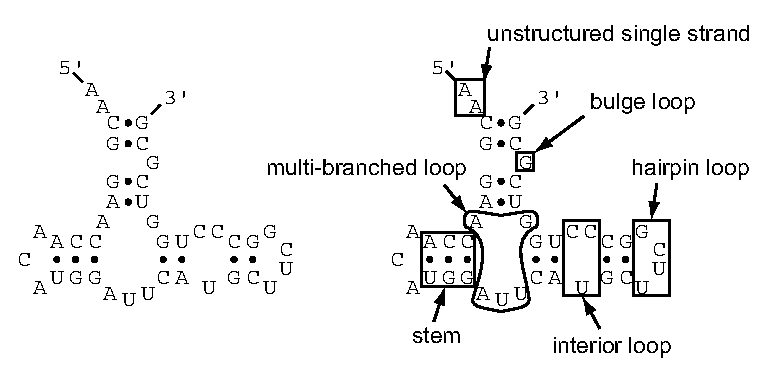
\includegraphics[scale=0.8]{figures/rna_elements}
\end{center}
\begin{center}
\begin{BVerbatim}
  ::((((,<<<___>>>,,,<<-<<____>>-->>,))-))
  AACGGAACCAACAUGGAUUCAUGCUUCGGCCCUGGUCGCG
\end{BVerbatim}
\end{center}

\subsection{Full (output) WUSS notation}

In detail, symbols used by WUSS notation in \emph{output} structure
annotation strings are as follows:

\begin{sreitems}{\textbf{Bulge, interior loops}}
\item[\textbf{Base pairs}]
  Base pairs are annotated by nested matching pairs of symbols
  \verb+<>+, \verb+()+, \verb+[]+, or \verb+{}+.
  The different symbols indicate the ``depth'' of the
  helix in the RNA structure as follows:
  \verb+<>+ are used for simple terminal stems;
  \verb+()+ are used for ``internal'' helices enclosing a multifurcation of
  all terminal stems; \verb+[]+ are used for internal helices
  enclosing a multifurcation that includes at least one annotated
  \verb+()+ stem already; and \verb+{}+ are used for all internal
  helices enclosing deeper multifurcations.

\item[\textbf{Hairpin loops}]
  Hairpin loop residues are indicated by underscores, \verb+_+.
  Simple stem loops stand out as, e.g.\ \verb+<<<<____>>>>+.

\item[\textbf{Bulge, interior loops}]
  Bulge and interior loop residues are indicated by dashes, \verb+-+.

\item[\textbf{Multifurcation loops}]
  Multifurcation loop residues are indicated by commas, \verb+,+.
  The mnemonic is ``stem 1, stem2'', e.g.\ \verb+<<<___>>>,,<<<___>>>+.

\item[\textbf{External residues}]
  Unstructured single stranded residues completely outside the
  structure (unenclosed by any base pairs) are annotated by
  colons, \verb+:+.

\item[\textbf{Insertions}]
  Insertions relative to a known structure are indicated by periods,
  \verb+.+. Regions where local structural alignment was invoked,
  leaving regions of both target and query sequence unaligned,
  are indicated by tildes, \verb+~+. These symbols only appear in
  alignments of a known (query) structure annotation to a target
  sequence of unknown structure.

\item[\textbf{Pseudoknots}]
  WUSS notation allows pseudoknots to be annotated as pairs of
  upper case/lower case letters: for example,
  \verb+<<<<_AAAA____>>>>aaaa+ annotates a simple pseudoknot;
  additional pseudoknotted stems could be annotated by \verb+Bb+,
  \verb+Cc+, etc. 

  This is not a fully general notation. It is possible to come up with
  pseudoknotted structures that could not be represented with 26
  levels of nesting ($>$26th order pseudoknot, in the sense of
  \citep{RivasEddy99}). However, it is unlikely you will ever see one
  in nature. I believe the highest order pseudoknot known is the S1
  (alpha operon) pseudoknot, which is 3rd order.
\end{sreitems}

An example of WUSS notation for a complicated structure
(\emph{E. coli} RNase P) is shown in Figure~\ref{fig:RNaseP}.  An
example of WUSS notation for a local alignment of \emph{B. subtilis}
RNase P to \emph{E. coli} RNase P, illustrating the use of local
alignment annotation symbols, is in Figure~\ref{fig:bsu-alignment}.

\begin{figure}[tp]
\begin{center}
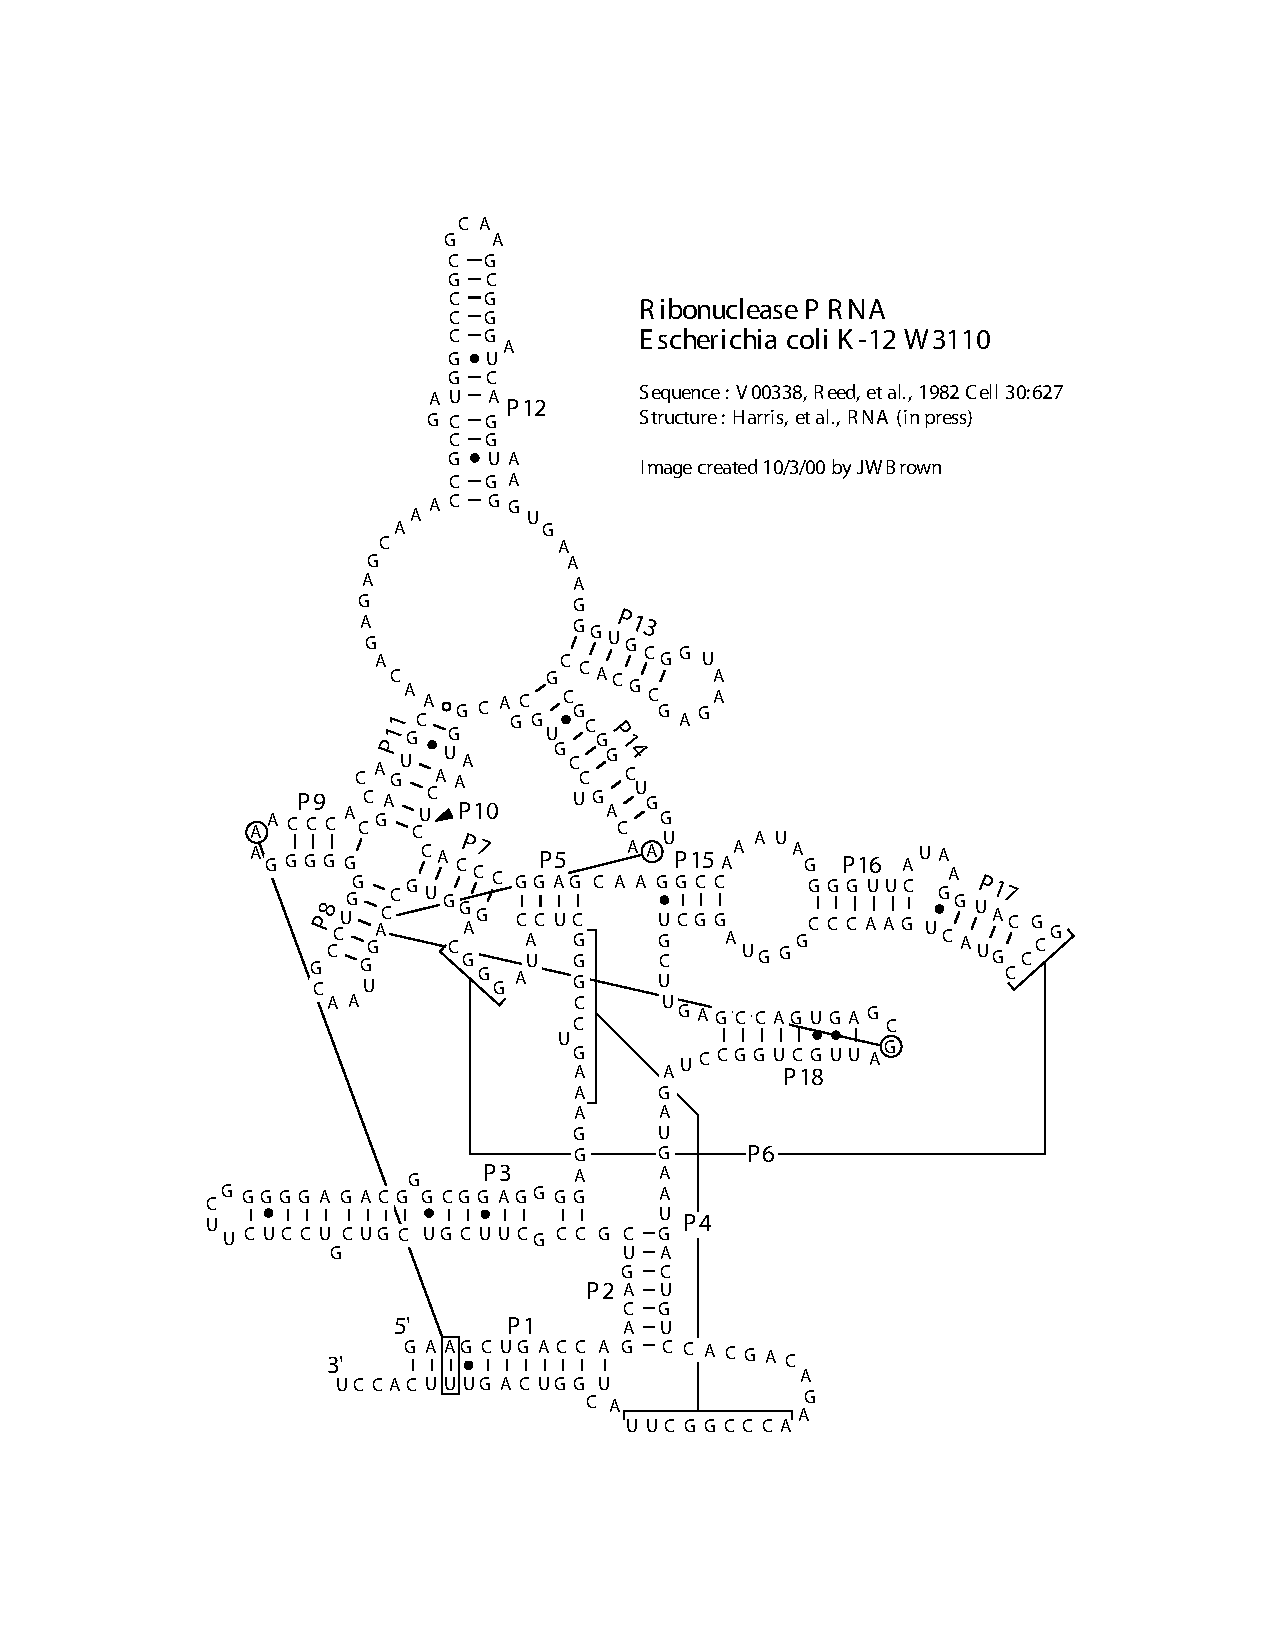
\includegraphics[scale=0.6]{figures/rnaseP-ecoli}
\end{center}
\begin{center}
{\scriptsize
\begin{BVerbatim}
           {{{{{{{{{{{{{{{{{{,<<<<<<<<<<<<<-<<<<<____>>>>>>>>>->>>>>>>>
         1 GAAGCUGACCAGACAGUCGCCGCUUCGUCGUCGUCCUCUUCGGGGGAGACGGGCGGAGGG 60

           >,,,,AAA-AAAAA[[[[---BBBB-[[[[[<<<<<_____>>>>><<<<____>>>->(
        61 GAGGAAAGUCCGGGCUCCAUAGGGCAGGGUGCCAGGUAACGCCUGGGGGGGAAACCCACG 120

           (---(((((,,,,,,,,,,,,<<<<<--<<<<<<<<____>>>>>->>>>>>-->>,,,,
       121 ACCAGUGCAACAGAGAGCAAACCGCCGAUGGCCCGCGCAAGCGGGAUCAGGUAAGGGUGA 180

           ,,,<<<<<<_______>>>>>><<<<<<<<<____>>>->>>>>->,,)))--))))]]]
       181 AAGGGUGCGGUAAGAGCGCACCGCGCGGCUGGUAACAGUCCGUGGCACGGUAAACUCCAC 240

           ]]]]]],,,<<<<------<<<<<<----<<<<<_bbbb>>>>>>>>>>>----->>>>,
       241 CCGGAGCAAGGCCAAAUAGGGGUUCAUAAGGUACGGCCCGUACUGAACCCGGGUAGGCUG 300

           ,,,,,<<<<<<<<____>>>>>>>>,,,,,,,,,,}}}}}}}----------aaaaaaaa
       301 CUUGAGCCAGUGAGCGAUUGCUGGCCUAGAUGAAUGACUGUCCACGACAGAACCCGGCUU 360

           -}-}}}}}}}}}}::::
       361 AUCGGUCAGUUUCACCU 377
\end{BVerbatim}
}
\end{center}
\caption{\small \textbf{Example of WUSS notation.} Top: Secondary
structure of \emph{E. coli} RNase P, from Jim Brown's RNase P database
\citep{Brown99}. Bottom: WUSS notation for the same structure,
annotating the \emph{E. coli} RNase P sequence. Note that the P4 and P6
pseudoknots are annotated, as A's and B's.}
\label{fig:RNaseP}
\end{figure}

\begin{figure}[tp]
\begin{center}
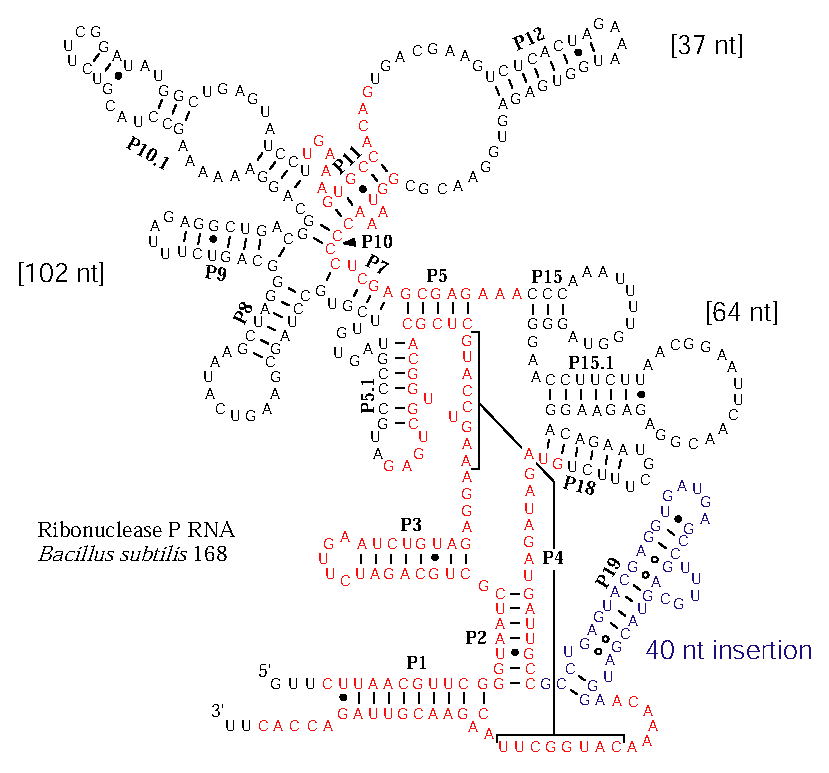
\includegraphics[scale=0.6]{figures/rnaseP-bsu-alignment}
\end{center}
\begin{center}
{\scriptsize
\begin{BVerbatim}
hit 0   :      4    399    52.56 bits
           {{{{{{{{{{{{{{{{{{,<<<<<<<<<<<<<-<<<<<____>>>>>>>>>->>>>>>>>
         1 ggAGuggGgcaGgCaguCGCugcuucggccuuGuucaguuaacugaaaaggAccgaagga 60
           +: :::G::C:GG:A:UCGCU+C::::            U+            ::::G+A
         4 CUUAACGUUCGGGUAAUCGCUGCAGAUC-----------UUG----------AAUCUGUA 42

           >,,,,,,,,,,,,,[[[.[--------[[[[[~~~~~~~((---(((((,,,,~~~~~~)
        61 GAGGAAAGUCCGGGCUC.CACAGGGCAgGGUG*[ 29]*GGAAAGUGCCACAG*[96]*G 229
           GAGGAAAGUCC  GCUC C  A GG   :G G       :GAAAGUGCCACAG      G
        43 GAGGAAAGUCCAUGCUCgC--ACGGUGCUGAG*[102]*UGAAAGUGCCACAG*[37]*G 226

           ))--))))]]]]]].]]],,,~~~~~~,,,,,,,,,,}}}}}}}--..............
       230 GUAAACCCCACCcG.GAGCAA*[77]*CuAGAUGAAUGacuGcCCA.............. 344
           GUAAACC:C C: G GAG AA       UAGAU++AUGA:U:CC
       227 GUAAACCCCUCGAGcGAGAAA*[64]*GUAGAUAGAUGAUUGCC--gccugaguacgagg 342

           ..........................-----------------}-}}}}}}}}}}::::
       345 ..........................CGACAGAACCCGGCUUAuagcCccaCUccucuu 377
                                       ACA AAC  GGCUUA:AG::C::: :+ C
       343 ugaugagccguuugcaguacgaugga--ACAAAACAUGGCUUACAGAACGUUAGACCAC 399
\end{BVerbatim}
}
\end{center}
\caption{\small \textbf{Local alignment annotation example.} Top:
Secondary structure of \emph{B. subtilis} RNase P, from Jim Brown's
RNase P database \citep{Brown99}. Residues in red are those that
Infernal aligns to a CM of \emph{E. coli} type RNase
P's. The local structural alignment is in four pieces; three regions
of the structure (102, 37, and 64 nt long) are skipped over. One
additional stem is treated as a 40 nt insertion. Bottom: the
Infernal output, showing the \emph{E. coli} query structure
aligned to the \emph{B. subtilis} sequence.}
\label{fig:bsu-alignment}
\end{figure}

\subsection{Shorthand (input) WUSS notation}

While WUSS notation makes it easier to visually interpret Infernal
\emph{output} structural annotation, it would be painful to require
people to \emph{input} all structures in full WUSS notation. Therefore
when software like Infernal reads input secondary structure
annotation, it also allows simpler rules:

\begin{sreitems}{\textbf{Single stranded residues}}
\item [\textbf{Base pairs}]
  Any matching nested pair of \verb+()+, \verb+()+, \verb+[]+, \verb+{}+
  symbols indicates a base pair; the exact choice of symbol has no
  meaning, so long as the left and right partners match up.
  Similarly, pseudoknotted pairs can also be annotated by matching nested
  pairs of any alphabet character, such as \verb+Aa+, \verb+Bb+, etc.

\item [\textbf{Single stranded residues}]
  All other symbols \verb+_-,:.~+
  indicate single stranded residues.
  The choice of symbol has no special meaning.
  Annotated pseudoknots (nested matched pairs of upper/lower case
  alphabetic characters) are also interpreted as single
  stranded residues in Infernal input.
\end{sreitems}

Thus, for instance, \verb+<<<<....>>>>+ and \verb+((((____))))+ and
\verb+<(<(._._)>)>+ all indicate a four base stem with a four base
loop (the last example is legal but weird).

Remember that the key property of canonical (nonpseudoknotted) RNA
secondary structure is that the pairs are \emph{nested}.
\verb+((<<....))>>+ is not a legal annotation string: the pair symbols
don't match up properly. 

Because many other RNA secondary structure analysis programs use a
simple bracket notation for annotating structure, the ability to input
the simple format makes it easier to use data generated by other RNA
software packages. Conversely, converting output WUSS notation to
simple bracket notation is a matter of a simple Perl or sed script,
substituting the symbols appropriately.


\newpage
\chapter{Appendix: design and construction notes}
\section{Tricks used to produce the documentation}

\subsection{autodoc - extraction of function documentation}


\subsection{cexcerpt - extraction of verbatim code examples}

This guide includes many examples of C code from Easel. These examples
are extracted verbatim from C source files using SSDK's
\prog{cexcerpt} program. The \prog{cexcerpt} program extracts tagged
code chunks from a C source file for verbatim inclusion in LaTeX
documentation.

The \ccode{documentation/Makefile} runs \prog{cexcerpt} on every
module .c and .h file. The cexcerpts are stored in the temporary
\ccode{cexcerpts/} subdirectory.

Usage: \ccode{cexcerpt <file.c> <dir>}. Processes C source file
\ccode{file.c}; extracts all tagged excerpts, and puts them in a file
in directory \ccode{<dir>}.

An excerpt is marked with special comments in the C file:
\begin{cchunk}
/*::cexcerpt::my_example::begin::*/
   while (esl_sq_Read(sqfp, sq) == eslOK)
     { n++; }
/*::cexcerpt::my_example::end::*/
\end{cchunk}

The cexcerpt marker's format is \ccode{::cexcerpt::<tag>::begin::} (or
end). A comment containing a cexcerpt marker must be the first text on
the source line. A cexcerpt comment may be followed on the line by
whitespace or a second comment.

The \ccode{<tag>} is used to construct the file name, as
\ccode{<tag>.tex}.  In the example, the tag \ccode{my\_example} creates
a file \ccode{my\_example.tex} in \ccode{<dir>}.

All the text between the cexcerpt markers is put in the file.  In
addition, this text is wrapped in a \ccode{cchunk} environment.  This
file can then be included in a \LaTeX\ file.

For best results, the C source should be free of TAB characters.
"M-x untabify" on the region to clean them out.

Cexcerpts can't overlap or nest in any way in the C file. Only one can
be active at any given time.




\newpage
\newcommand{\bibfont}{\footnotesize}
\bibliographystyle{apalike}
\bibliography{master,lab,books}

\end{document}

